\documentclass{article}
\usepackage[utf8]{inputenc}

\usepackage[english]{babel}
\usepackage{parskip}
\usepackage{tablefootnote}
\usepackage[nottoc]{tocbibind}
\usepackage{amssymb}
\usepackage{mathtools} 
\usepackage{geometry}
 \geometry{
 a4paper,
 total={140mm,227mm},
 left=35mm,
 top=35mm,
 }

\usepackage{float}
\usepackage{graphicx}
\usepackage{epstopdf}
\usepackage{amsmath}
\usepackage{bm}

%dank
\usepackage{marvosym}

\setlength{\parindent}{0pt}
\numberwithin{figure}{section}
% equation number format: in section 1, (1.1), (1.2) ..
\usepackage{amsmath}
\numberwithin{equation}{section}

\makeatletter
% we use \prefix@<level> only if it is defined
\renewcommand{\@seccntformat}[1]{%
  \ifcsname prefix@#1\endcsname
    \csname prefix@#1\endcsname
  \else
    \csname the#1\endcsname\quad
  \fi}
% define \prefix@section
% \newcommand\prefix@section{}
\makeatother

%% multi col
\usepackage{multicol}

\usepackage{siunitx}

\usepackage[colorlinks]{hyperref}

% hyperlinks
\usepackage{hyperref}
\hypersetup{
    colorlinks=true,
    linkcolor=black,
    citecolor=red,
    urlcolor=blue,
    filecolor=red,
    bookmarksopen=true
} 
\urlstyle{same}


% colored frames (boxes)
\usepackage{xcolor}
\usepackage{mdframed}

% vector arrow with \vv{ }
\usepackage{esvect}

%\hyphenpenalty 10000
%\exhyphenpenalty 10000
%\usepackage[none]{hyphenat}
%\usepackage[document]{ragged2e}

% strike through text
\usepackage[normalem]{ulem}
% \sout{Hello World}

\usepackage{listings}
\lstset{language=Java,
basicstyle=\ttfamily,
keywordstyle=\color{blue}\ttfamily,
stringstyle=\color{red}\ttfamily,
showstringspaces=false,
commentstyle=\color{purple}\ttfamily,
morecomment=[l][\color{magenta}]{\#}, 
%numbers=left,
numbersep=5pt, 
backgroundcolor=\color{white}, 
breaklines=true
}

\usepackage{siunitx}
%\usepackage{unixode}


% spacing in enum and itemize
\usepackage{enumitem}

% \usepackage{slantsc}
\usepackage{bold-extra}
% New commands 



\newcommand{\C}{\textcircled{}}
\newcommand{\CT}{\textcircled{$\checkmark$}}

\usepackage{caption}
\usepackage{subcaption}


%%%%%%%%%%%%%%%%%%
%% HEADER OVER %%%
%%%%%%%%%%%%%%%%%%

\begin{document}
\pagenumbering{gobble}

\title{02122 Software Technology Project: IBM Netbank Case}
\author{\textbf{Group 4:} \\ 
s144063	Magnus Middelboe Søborg-Madsen \\
s151952	Jens Carl Moesgård Eschen \\
s154666	Mikkel Clausen Knudsen \\
s144107	Roar Nind Steffensen}
\date{\today}

\maketitle

\begin{figure}[H]
    \centering
    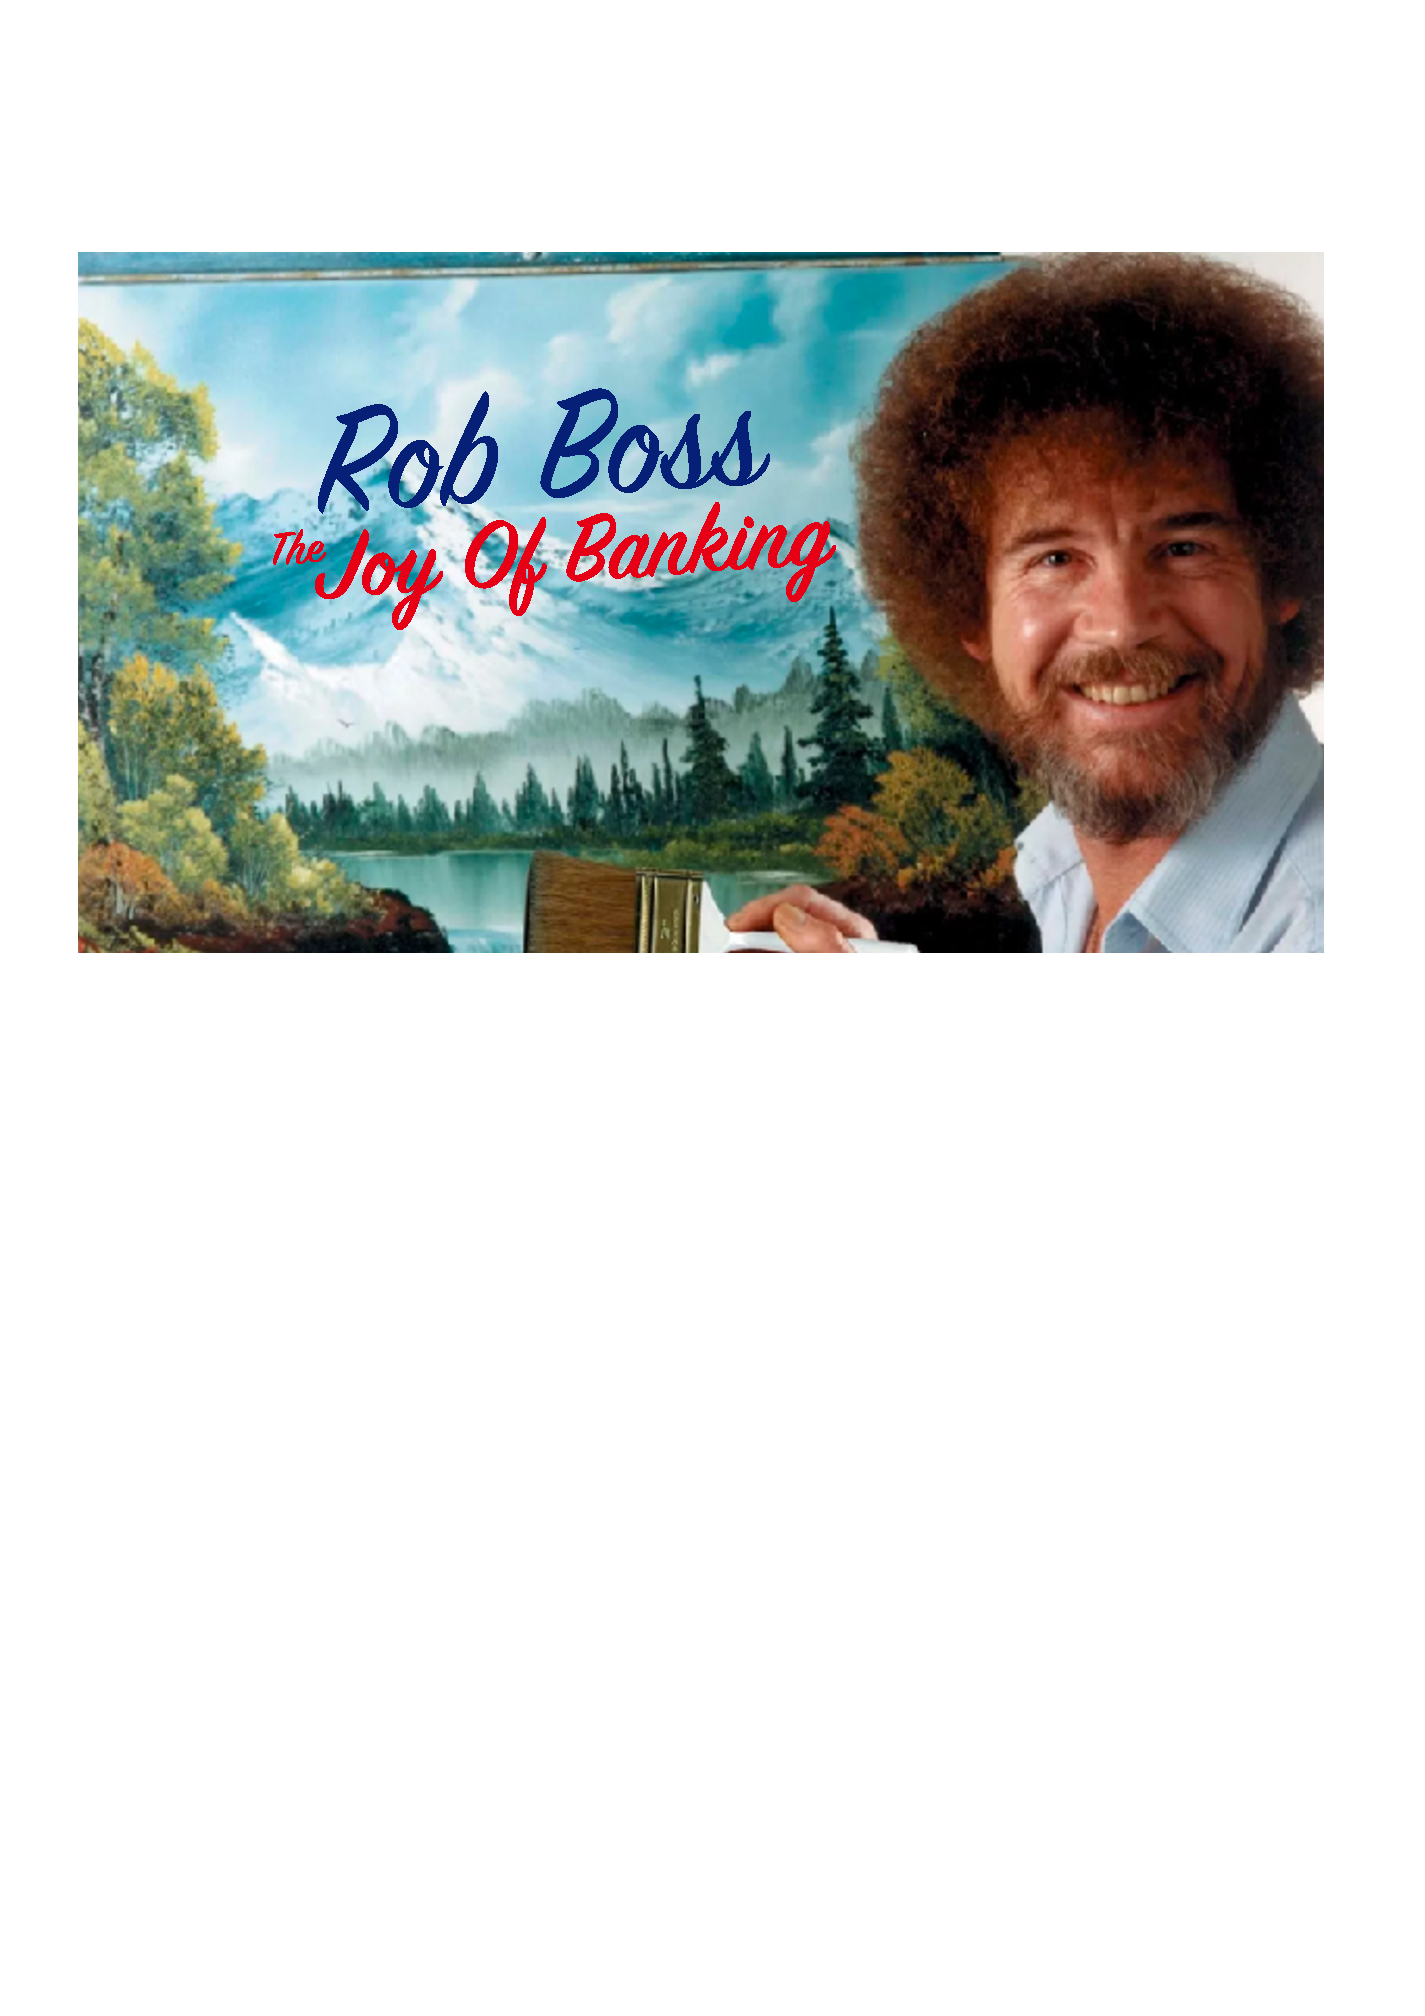
\includegraphics[width=\linewidth]{figures/Gruppe4_logo.pdf}
    \label{fig:logo}
\end{figure}

\begin{figure}[H]
    \centering
    
\includegraphics[width=0.8\linewidth, height=18mm]{figures/underskrifter.png}
    \label{fig:underskrifter}
\end{figure}

% \begin{mdframed}[backgroundcolor=black!5]
% Der skal være en forside indeholdende: navne på forfatterne (gerne studienumre),
% gruppenummer, dato, titel.  \\
% • Rapporten skal være forsynet med jeres underskrifter. \\

% Af hensyn til den individuelle bedømmelse skal der for hvert kapitel/afsnit
% angives, HVEM der har produceret indholdet. Der må kun stå ét navn

% %Logins til Maria, Henrik, Paul, Nina, admin
%  \end{mdframed}
\vfill

\begin{center}

%{\normalsize Logins:}

 \begin{table}[H]
     \centering
     \begin{tabular}{l|c|c}
        \textbf{Name} & \textbf{Username}  &  \textbf{Password} \\ \hline
        Maria Kroos Boisen  & maria  & maria \\
        Henrik Thorsen  & henrik  & henrik \\
        Paul Fischer  & paul  & paul \\
        Nina Gierasimczuk  & nina  & nina \\
        admin  & admin  & admin \\
     \end{tabular}
 \end{table}
 
 {\Large  \url{http://192.86.32.54:9080/RobBossv04/} }

 
\end{center}



\section*{Abstract (Roar)}

\textit{In this project, we have developed an online bank application using the Model-View-Controller design pattern. The design and implementation is outlined and discussed with emphasis on the development decisions the applications has undergone.}

\textit{The applications makes use of a variety of tools provided by IBM: Data Studio, DB2 Database and WebSphere Application Server Liberty Profile and a z13 mainframe running z/OS. Self-provided tools include Java, Git, JSP and JUnit.}

\textit{Automatic and functionality tests have been used to verify the quality of the application, with respect to robustness and user experience. Feedback from a focus group has been received and taken into consideration with regards to UI interaction.}

\textit{The final product satisfies a set of specified requirements mainly provided by IBM, and the focus group was able to perform a list of necessary tasks, comprised of what is expected from an online bank.}

\setcounter{tocdepth}{2}
\tableofcontents

\vfill

\textit{Robert "Bob" Ross was a painter, television host, and internet celebrity.
For decades, he hosted the American TV show The Joy of Painting, a show dedicated to landscape oil painting in a relaxing setting. Bob Ross is attributed the quote "There are no mistakes, only happy accidents."}

\textit{When creating the logo and name of the bank, we chose the bank name Rob Boss to highlight the joy of using our net bank, just as Bob Ross highlighted the joy of painting. To avoid copyrights, we switched the initials. Ironically, these switched initials ended implying that the bank is a boss of robbing its customers.}

\newpage

\pagenumbering{arabic}
\setcounter{page}{1}

\setcounter{tocdepth}{2}


\section{Introduction}

%\subsection{Intro (0.1 p) (Magnus)}
In DTU course 02122 Software Technology Project, the overall task is to develop, evaluate and document a larger software project. This report documents how we developed, tested and evaluated an online bank application in collaboration with IBM Denmark.
\subsection{Context (Magnus)}
Denmark is one of the most digitized countries in the world, and \#1 in EU\cite{danmark_mest_digi}. The promise is that this will increase productivity\cite{digitalisering_oeger_produktivitet}.  The online bank is an increasingly important aspect of a bank. When customers choose a bank, the online bank is more important than the assigned in-person counsellor\cite{netbank_raadgiver}. Danish customers prefer to manage their day-to-day banking through the online bank, rather than going to the physical bank\cite{netbank_foretrukken}. 88 \% of Danes use online banks\cite{danskere_bruger_netbank}, hence millions non-technical users (and billions worldwide) rely on secure and easy-to-use online bank applications.


\subsection{Motivation (Magnus)}
We chose this project mainly for three reasons: First, to gain experience with solving a real-life technical problem while focusing on customer requirements.

Second, to apply knowledge acquired in DTU courses (e.g. Java, Git), and get experience with independently seeking out knowledge required in e.g. SQL and HTML. 

Third, IBM is one of the biggest players in the IT market\cite{wikipedia_it_companies} and a top-10 Fortune 500 company in the technology sector\cite{fortune500}, so the project aligns well with DTU's strategy to work closely with the business community\cite{dtu_strategy}.
\subsection{Goals (Magnus)}
The overall goal is to \textit{create a realistic online bank}, using common approaches and tools, i.e. tools that we can expect to encounter after graduating from DTU.

We focused on some non-functional requirements:
\begin{itemize}
\setlength\itemsep{0em}
\item \textbf{Usability} (ease-of-use): Users should have an easy time using the online bank.
\item \textbf{Extensibility}: The application should be easy to develop further.
\item \textbf{Simplicity}: The application should have a clear structure, the code should be readable.
\item \textbf{Scalability}: The data structure should handle growth in size appropriately.
\item \textbf{Security}: With money involved, it is essential to guard against malicious use.
\end{itemize}

We were also given 11 requirements in the problem assignment, to emulate requirements given set by a customer. These are presented in section  \ref{sec:problemanalysis_requirements}.
\subsection{Evaluation (Jens Carl)}
Our evaluation of the application will be twofold. It will not only contain automated tests to confirm the inner workings of the back-end, but also front-end focus testing by volunteers. They will be given a task list. Since ease-of-use is a main design metric, the time it takes for them to complete it will be recorded. Together with the automated tests, the average time used will be our central measurement in the evaluation of the success of the project. 

%How to evaluate program: real-life test subjects
%We chose to evaluate the application in two ways: str

%\subsection{Summary of overall conclusion (0.2 p)}


%% PROB ANA AND REQ START
\section{Problem analysis and requirements}\label{sec:problemanalysis_requirements}
\subsection{Problem analysis (Mikkel)}

% \begin{mdframed}[backgroundcolor=black!5]
% Opgavebeskrivelse og -analyse
% Ud over det i noten nævnte er det nærliggende at analysere opgaven i et omfang så der
% er lagt op til den efterfølgende kravspecifikation.
%  \end{mdframed}

The assignment description, as given in the case description by our IBM supervisors, can be seen below. Note that the description has been translated from Danish\cite{case_description} to English.

%% DEEL AF TESK 
%% IKKE SLET
\begin{mdframed}[backgroundcolor=black!5]
A bank - DTU Bank A/S - situated in Lyngby are in the process of buying banks around the world. This poses new and bigger demands to their IT system - both in the infrastructure and on the application level. DTU Bank A/S have therefore chosen to develop an entirely new banking system on an IBM enterprise server.
%En bank - DTU Bank A/S - med hovedsæde i Lyngby er i færd med at opkøbe banker rundt om i verden. Det stiller nye og større krav til deres IT system - både infrastruktur og på applikations niveau. DTU Bank A/S har derfor valgt at udvikle et helt nyt kontosystem på en IBM entreprise server
\end{mdframed}
%% DET ER MENIngEN
 %% IKKE SLE
 
From this followed a number of requirements for the program. 

\subsection{Requirement specification (Mikkel)}

% \begin{mdframed}[backgroundcolor=black!5]
% Definerer væsentlige begreber indenfor problemdomænet og
% afgrænser opgaven som skal løses. \\
% Angiver funktionelle og ikke-funktionelle krav.
% Kravene bør være testbare.
% Disse kapitler skal kunne læses af \\
% • “kunden” og af \\
% • medstuderende/personer der skal vedligeholde jeres system. \\

% De næste 2 afsnit udgør bindeledene mellem kravspecification og kildekoden. \\

% Kravene bør \textbf{prioriteres}, så man kan se, hvad der er vigtigst at få implementeret hvis
% man kommer i tidnød senere, og ikke kan nå at lave alt. Kravene skal nummereres, se
% de let kan refereres i forbindelse med test. Det bør også klart fremgå "hvilket krav der
% kommer af hvad", f.eks ved at liste brugsscenarier og under hvert scenarie angive de
% afledte krav. Kravene bør være testbare ellers kan man jo ikke godtgøre at det færdige
% produkt opfylder kravspecifikationen. Hvordan fejlhåndteringen skal være kommer også
% naturligt ind her.
%  \end{mdframed}

Requirements are given already in the assignment specification \cite{case_slides}, and can be seen below. The specifications have been translated, as well as reordered and divided into groups.\\

%% IKKE TEMPPORERY
%% IKKE LSSTET
\begin{mdframed}[backgroundcolor=black!5]
\begin{enumerate}
\item[$ $] \textbf{Users and accounts:}
\item Create a new account for a user in the banking system.
%\item Oprette en ny konto for en person i en given medlemsbank. 

\item Edit information about the individual accounts, such as rate of interest.
%\item Rette oplysninger om den enkelte konto (renteprocent, evt, navn på ejer)

\item Delete an account, taking into consideration circumstances such as remaining account balance, debt, and so forth.
%\item Nedlægge en konto, med de forholdsregler som bør tages i forhold til eksisterende saldo, gæld, etc.

\item Show transaction history for the current week, as well as showing the account balance for a customer in the bank.
%\item Visning af transaktioner for indeværende uge samt saldo på konto for en given bankkunde

\item[$ $] \textbf{Transactions:}

\item Perform insertions of money into an account, while keeping track of the account balance, and storing the transaction.
%\item Udføre indsættelser  af beløb på konto (ajourføring af saldo og lagring af transaktion)

\item Perform extractions of money from an account, while keeping track of the account balance, and storing the transaction.
%\item Udføre udtog på konto (ajourføring af saldo og lagring af transaktion)

\item Make sure an account never goes below 0,- and reject transactions that would make it go below 0,-.
%\item Kontrol med, at en konto aldrig går under 0,-. En sådan transaktion skal afvises


\item[$ $] \textbf{Currency:}

\item Translate money from one currency to another for transactions.
%\item Valutaomregning i forbindelse med transaktioner, hvis transaktionen foregår uden for kundens hjemland

\item Be able to specity which currency to show account balance and transaction history.
%\item Muligheden for at specificere i hvilken valuta, saldo og bevægelser skal vises.

\item[$ $] \textbf{Maintenance and scalability:}

\item Perform a batch-solution to archive transactions that are more than a week old.
%\item Der skal endvidere udvikles en batch-løsning, som en gang om ugen kan arkivere ugens transaktioner på en arkiv-database, således at kun de nyeste transaktioner vises.

\item The system must be scalable, and effectively be able to handle a million accounts.
%\item Systemet skal være skalerbart og effektivt kunne håndtere en million konti
\end{enumerate}

\end{mdframed}
%% DET ER EN DEL AF RAPPORTS
%% DO NOT ELST

Besides these, we added two requirements to the program.

\begin{enumerate}
    \item[$12.$] It must be intuitive to use, such that someone with no prior knowledge of the program can figure it out in 10 minutes or less, without guidance.
    \item[$13.$] It must have at least a minimum of security, such as passwords being stored safely, and protection from SQL injection.
\end{enumerate}

%Most of these, we implemented directly, such as translating from one currency to another. 

We chose to have the primary login for a user to go to a 'Customer' page, instead of having each individual account have a separate login. This made it so the functionality requirements relating to accounts have been re-purposed to work on all accounts a user has, as well as the individual account. 

Requirement nr. 2 has been reinterpreted to incorporate administrative users. It is only administrative users that are able to edit certain account information, such as rate of interest. The customer is still able to edit which currency to show their account balance and transaction histories in.

Requirement nr. 7 has been reinterpreted to incorporate credit for an account, allowing it to have a balance below 0,- as long as it has remaining credit in the bank. Similarly, a transaction that would make the account balance go below the account's specified credit will be denied. All accounts start with a bank credit of 0,- as in the functionality requirements, but can be changed by an administrator if necessary. 

The batch-solution is not automated, but instead must be performed manually by an administrator on the system.


%% PROB ANA AND REQ END

%% IBM & GIVEN TOOLS START
\section{IBM}\label{sec:ibm}
%\subsection{Intro (0.1 p)}
In this section, we present important tools and terms related to IBM and this project.

\subsection{The Mainframe (Jens Carl)}

The mainframe is a large computer  used by big corporations. Multiple systems can be run on the mainframe, and its memory segment can be divided into many independent and isolated logical partitions.

The mainframe has for a long time been one of IBM's signature products\cite{ibm_history_slides}. One of the trademarks of modern IBM mainframes is their extremely high up-time and stability\cite{red_book}. For storage of very important information often accessed (e.g. money), these properties are a must. 

\subsection{DB2 (Magnus)}
DB2 is a database tool made by IBM. Like other popular database tools, it is relational, i.e. an RDBMS (\textbf{R}elational \textbf{D}ata\textbf{b}ase \textbf{M}anagement \textbf{S}ystem). We use DB2 to store, modify and retrieve data in a database on a z/OS partition on the Mainframe. DB2 can trace it roots back to IBM researcher by E. F. Codd, whose 1970 paper \textit{A Relational Model of Data for Large Shared Data Banks}\cite{codd} paved the way for the relational database systems in general.

\textbf{Why use DB2?} DB2 is one of the most used database management systems in the world\cite{db2}. While MySQL is free, IBM offers extensive customer support for DB2. DB2 is an IBM product and performs well on z/OS. The DTU course 02170 on database systems uses MySQL instead of DB2, but both systems support the SQL standard. We contacted lecturers of course 02170, and self-studied some SQL.

To access and modify the DB2 database we use the tool Data Studio.
\subsection{z/OS (Magnus)}

z/OS is a 64-bit operating system made for IBM mainframes. It supports the other tools used in this project (DB2, Java), but also popular tools like C and COBOL. The Mainframe supports several z/OS partitions to run concurrently with no access to another partition's memory.

\textbf{Why use z/OS?} It is used by Danske Bank, the largest bank in Denmark\cite{danske_pengeinstitutter}. Our online bank application only has $\approx$ 10 users and $\approx 1$ transaction per second, so a household server could host our application. But running the online bank application on the IBM mainframe on a z/OS OS provides \textit{proof of concept} that our application can run on commercially used hardware.
\subsection{Sysplex (Jens Carl)}
% Sysplex is short hand for Systems Complex
Sysplex is the short hand for the IBM term \textit{Systems Complex}. It consists of multiple z/OS images linked together to a single operational unit. These images can also be distributed across different mainframes and coupled together with  \textit{Coupling Facilities}. Using the same shared data, this (called a \textit{Parallel Sysplex}) provides a multitude of business-relevant features such as:
\begin{enumerate}
    \item Continuous availability through maintenance and changes to the system. 
    \item Excellent disaster management in case of outage.
    \item Dynamically balanced workload for high performance. 
\end{enumerate}
%\input{ibm/redbook.tex}
%% IBM & GIVEN TOOLS END

\section{Use cases (Jens Carl)}
\label{sec:usecases}
%\subsection{Use cases (1 p) (Jens Carl)(draft 1)}
In the process of turning the requirement specification into a fully fledged bank application, we started off developing use cases to get a better understanding about the scope of the program. Later these use cases were used as central points in the design phase. For an overview see figure \ref{fig:usecases}. Below is an example of a use case.

\subsubsection{Use case example: Performing a transaction}
\begin{itemize}
    \item[--] name: Transfer money
    \item[--] actor: customer (user)
    \item[--] main scenario: transferring money
        \begin{enumerate}
            \item User logs in.
            \item User fills out receiver field, which can either be another customer or an account id. 
            \item User selects account to transfer from.
            \item User enters amount to transfer in units of currently preferred currency.
            \item User clicks "transfer money". 
            \item Money is moved from users account.
            \item A transaction is displayed in the transaction history table. 
        \end{enumerate}
    \item[--] alternative scenario:  wrong receiver input
        \begin{enumerate}
            \item User enters a username or account id which does not exist.
            \item An error message is displayed at the top of the page. 
        \end{enumerate}
    \item[--] alternative scenario: insufficient funds
        \begin{enumerate}
            \item User enters a value larger than the amount available on their selected account. 
            \item An error message is displayed at the top of the page. 
        \end{enumerate} 
\end{itemize}
\begin{figure}[H]
    \centering 
    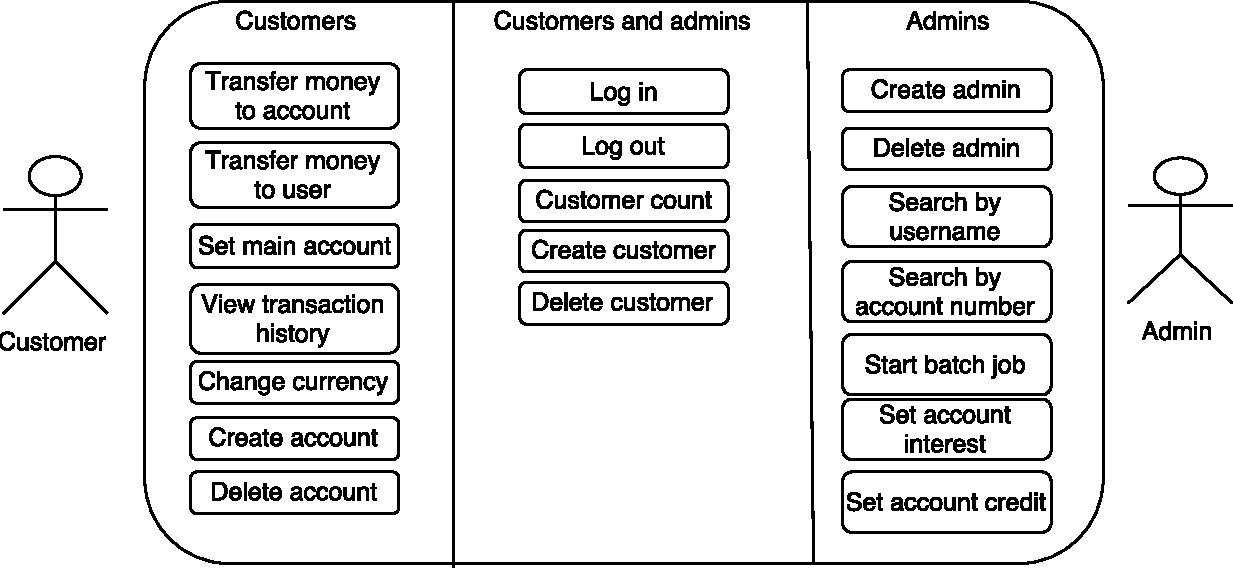
\includegraphics[width=\textwidth]{figures/use_case_diagram_final.pdf}
    \caption{Figure illustrating the different use cases. There are two different types of users; bank employees (administrators) and customers. Both users have some use cases in common, e.g. logging in and out of the application. Other cases are only preformed by one of the two. Customers need to manage their accounts and transfer money around. Admins needs to manage user profiles and account settings and perform maintenance.}
    \label{fig:usecases}
\end{figure}


%% DESIGN SECTION START
\newpage
\section{Design}
\label{sec:design}
%\subsection{Intro (0.1 p)}

In this section, we cover the tools used, the design pattern we chose,  the general architecture of the application, as well as the security measures taken into consideration while designing the application.


\subsection{Tools (Magnus)}\label{sec:tools}

First we present the tools used, complementing those in the IBM section (the mainframe, z/OS, DB2). Then we reflect on the advantages and disadvantages of each. 

The tools used in this project were given, and are seen in Fig \ref{fig:communication_external}. In short: The application is written in \textbf{Java}, and runs on a \textbf{z/OS} operating system on an \textbf{IBM mainframe}. The customer data is stored in a \textbf{DB2 database}, also in the mainframe. The user interacts with the application through a \textbf{web browser} e.g. Chrome. We chose to build the web pages with \textbf{JSP}.

\textbf{Why use Java?} Java has a vast set of libraries that makes implementation fast. Java runs slower than e.g. C, but has no buffer overflow. We have experience with Java from DTU course 02101. Eclipse offers Git tools for version control. Java is a language used on the Danske Bank IBM mainframe, so it is a valid real-life choice \cite{danskebank_java}.

 

\textbf{Why use JSP?} \textbf{J}ava\textbf{S}erver \textbf{P}ages is a technology that integrates Java code and HTML. This means we could apply our knowledge of Java when creating web pages. There are other popular technologies for building web pages, but as we have little experience with web development, JSP seemed like a good choice. We had to self-study some HTML, but as HTML the most popular markup language for web pages \cite{html_most_used}, this was good time investment.

\begin{figure}[H]
\centering
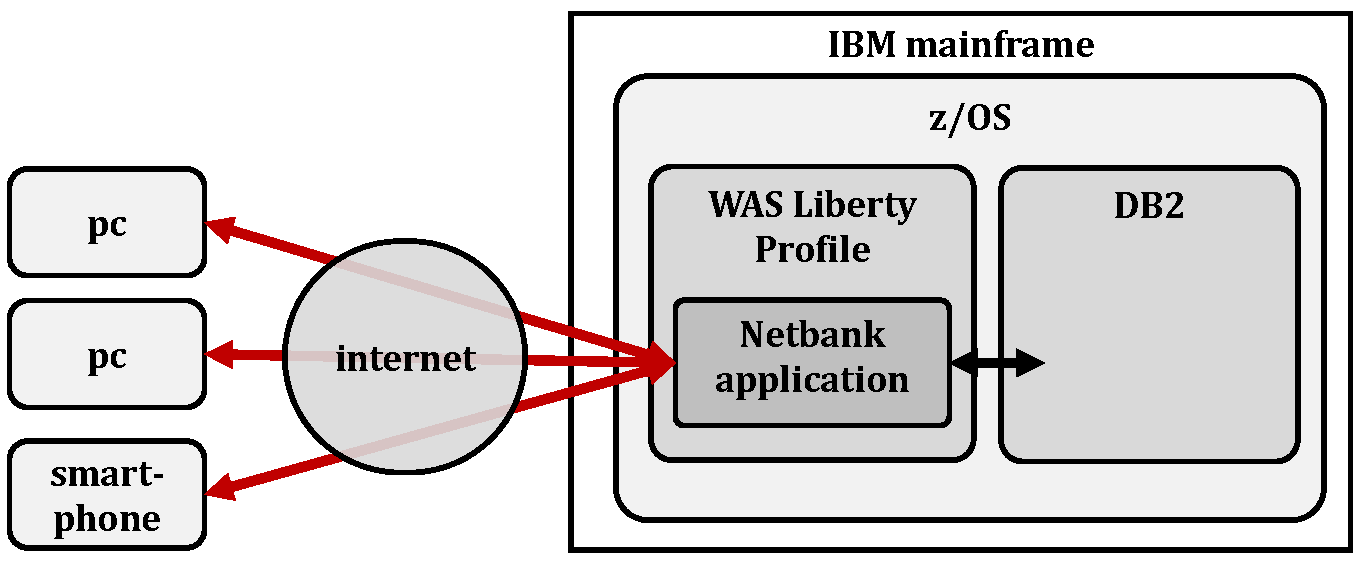
\includegraphics[width = 0.7\textwidth]{figures/communication1.pdf}
\caption{Commutation chart, when the application is running on the IBM Mainframe.}\label{fig:communication_external}
\end{figure}


\subsection{Model-view-controller (Jens Carl)}
We chose to develop our application from the Model-view-controller design pattern. For an overview of MVC and our class implementation see figure \ref{fig:MVC_CD}

The MVC design pattern is our team's most familiar design/architecture pattern to develop from. We've used it, and been taught it, in past projects in previous courses\footnote{DTU courses 02121 Intro to Software Tech, 02161 Software Engineering 1} to great success. The MVC pattern is simple to implement in group-work since work on independent parts can be split up. During development it helps keep up the workflow with either a top-down approach (starting from the controller and working downwards towards the elementary data model) or bottom-up (implementing the data model first and then using it in controller methods). For long term development, the MVC provide relatively good flexibility for changing plans (e.g. changing data structure) mid-term. The old model can be reused for a different purpose by re-routing in the controller, and previously made view classes (front-end) can remain mostly unchanged while the back-end is reworked.  
All in all, choosing MVC provides us with an experienced starting point and fits well into the scope of the project.

\begin{figure}[H]
\centering
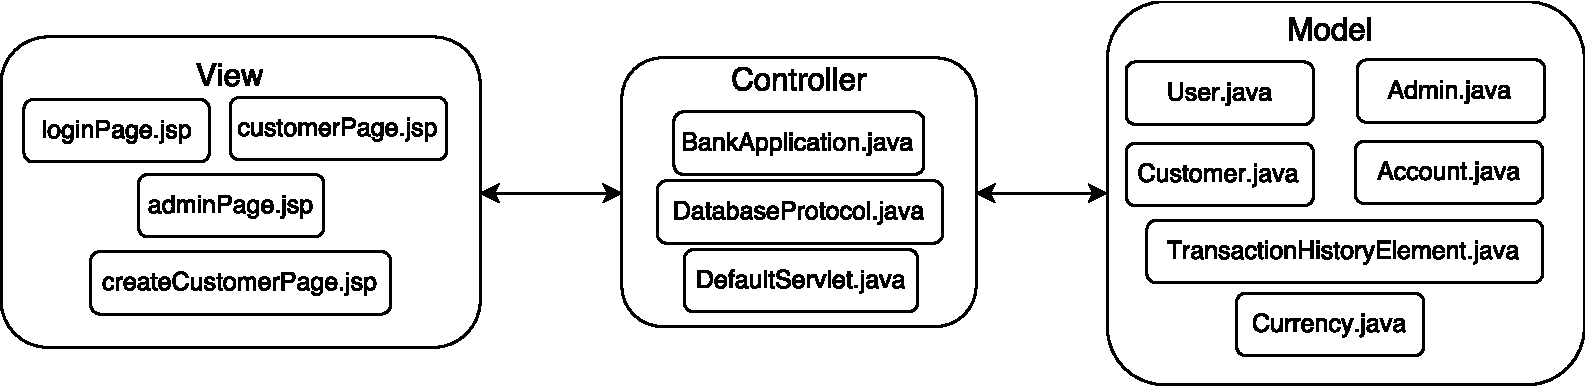
\includegraphics[width = 1.00\textwidth]{figures/class_diagram_abridged.pdf}
\caption{Diagram showcasing how we divided our classes into the three MVC components. The web layout files are in the View component. They register user input and send it to the Controller. The controller consist of Java classes governing the main logic in the application. Based on the signal from View, it tells the Model which changes in data that need to occur. Data in the Model can in turn provoke the Controller to make new changes, and in the end the Controller sends back to View what should be displayed to the user.}
\label{fig:MVC_CD}
\end{figure}
\subsection{Model design (Jens Carl)}
% Main classes: User, Customer, Admin, Account
% Wrapper-ish: TransactionHistoryElement, Valuta
%
% Points:
% We looked at existing net banking applications
% and used them as inspiration. 
% We also used our own experience and intuition
% to build the data model.
% 
% Starting with an idea of logging in as an user % through a webapplication helped us grasp the 
% problem domain and get a good starting point.
%
% From there on the model began forming itself
% - It became evident that out vision of being 
%   a user was split into two parts: customer and
%   admins. 
% - A user is an abstract entitiy that can either %   take shape as an admin or as a customer.
% - 
%Starting with an idea of logging in as an user through a webapplication helped us 

%we wanted the data model to mimic the beheavior of the subject at hand: the user of the application. Therefore we want an abstract entity 'User' which can take form as either a 'Customer' or an administrator 'Admin' logging on. 
%The person using the application (e.g. user).Wether this user is a customer of the bank, or an intern working as an administrator (e.g. admin). His/Hers potential accounts. And last, but not least, other users and accounts \begin{itemize}
%    \item The person using the application %(e.g. user).
%    \item Wether this user is a customer of the bank, or an intern working as an administrator (e.g. admin).
%    \item His/Hers potential accounts.
%\end{itemize}to interact with.
%\begin{itemize}
%    \item[--] Users; members of the bank. Core information about users must be stored in the database. This includes login credentials (username, password) and a name.
%    \item[--] Customers. If a user is a customer, linkage to his/hers account(s) must also be stored, along with customer-unique preferences. 
%    \item[--] Admins. If a user is an administrator, working at the bank, his/hers    
%    \end{itemize}
% Designing on an object-oriented basis, we took key elements in the problem domain and devided them into objects:
% \begin{itemize}
%     \item[--] Users; members of the bank. Core information about users must be stored in the database. This includes login credentials (username, password) and a name. There are two kinds of users:
%     \begin{itemize}
%         \item[--] Customers; possesing accounts and unique preferences. 
%         \item[--] Admins; no extra data other than the type. 
%     \end{itemize} 
%     \item[--] Accounts; 
% \end{itemize}
%Thus, our model takes its starting point in the thought of frequent fetching/storing from/to a database.

%introduction
The database was an essential part of the model component of MVC. It provides the ability to store information between sessions, which can be accessed by computers with a connection. For an online banking application, this is exactly what's needed. 

When designing the table structure of the database, we mirrored elements in the problem domain: We wanted customers, accounts and admins to be the core entities in the application, so we made tables for those. See figure \ref{fig:wackyModelDesign}.
\begin{figure}[!htb]
    \centering
    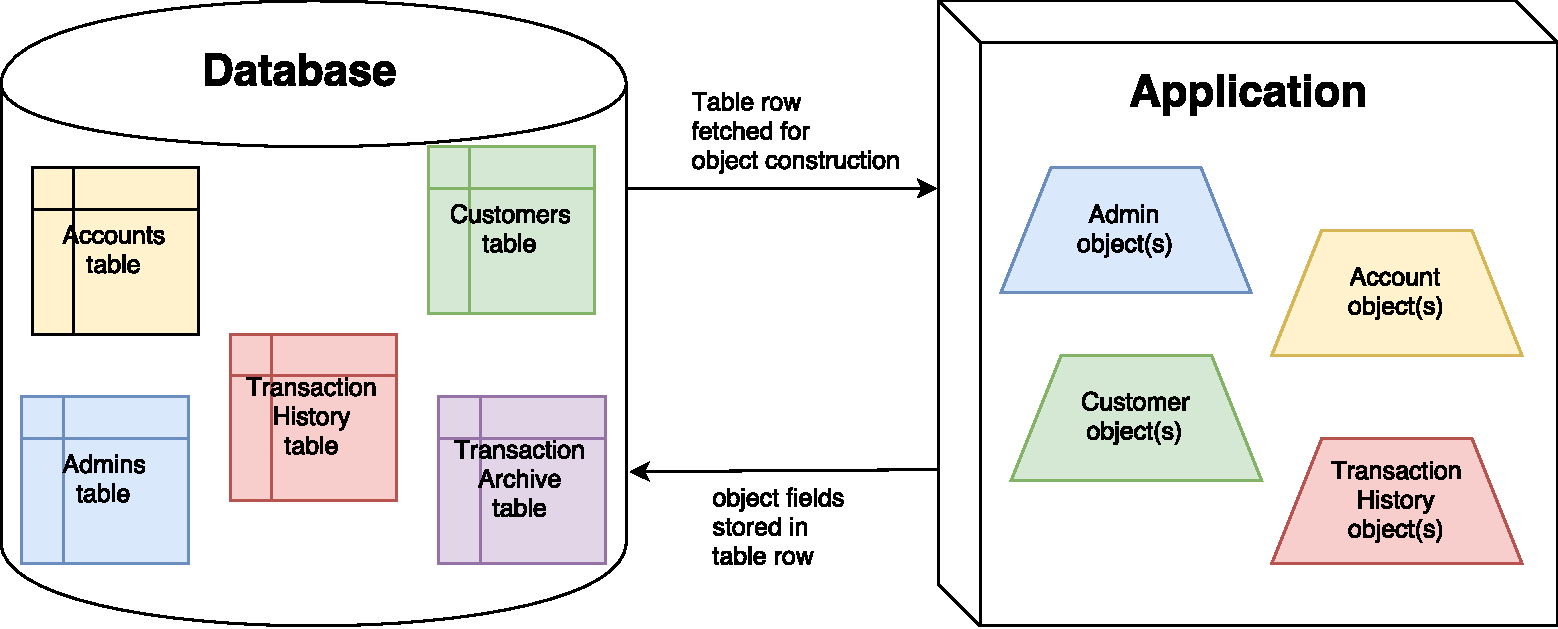
\includegraphics[scale=.5]{figures/modelDesign.pdf}
    \caption{Figure illustrating how the model is designed with the database in mind. Designing on an object-oriented basis, we took key elements in the problem domain and divided them into sections. There are 'Customers' of the bank with  bank 'Accounts'. Their transactions are stored in the 
    'Transaction History'. Lastly there are also 'Admins' working at the bank, with special privileges.}
    \label{fig:wackyModelDesign}
\end{figure} 

In the application, the model is almost mirrored the database, except that instead of storing \textit{every} customer, only a few relevant are stored locally each session of use. Objects are constructed with the information provided in a given row of the tables, and they're modified during the session of user interaction. When changes are committed, the data in the same objects are stored in their corresponding table rows.
\subsection{View design (Magnus)}\label{sec:viewDesign}

We settled on the following four pages as part of the View (Fig \ref{fig:MVC_CD}): a login page, a create customer page, a customer page, and an admin page. For sample screenshots of these pages, see Appendix \ref{sec:appendixView}. Adhering to the MVC design pattern, these pages should be limited to presenting the current Model data. The user interacts with the application through a web browser. All communication with the Model should occur through the Control classes.

\begin{figure}[H]
\centering

\begin{subfigure}[b]{0.49\textwidth}
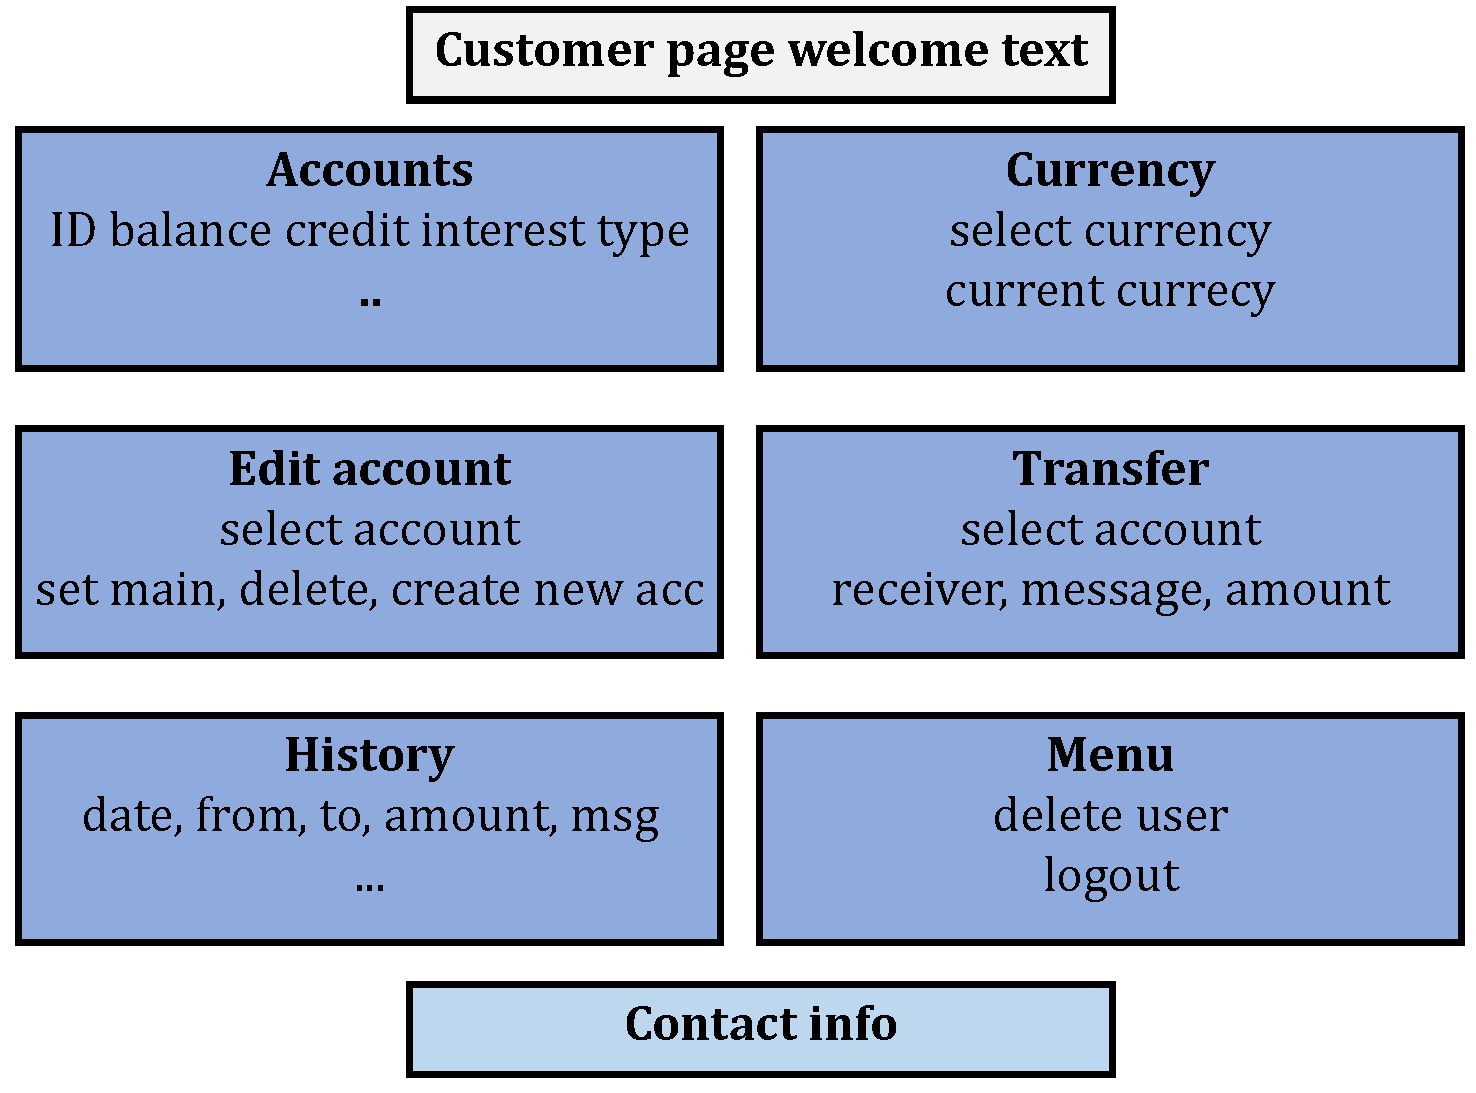
\includegraphics[width=\textwidth]{figures/customerPage.pdf}
\caption{Intended content in the customer page.}
\label{fig:customerPageDesign}
\end{subfigure}%
\hfill
\begin{subfigure}[b]{0.49\textwidth}
  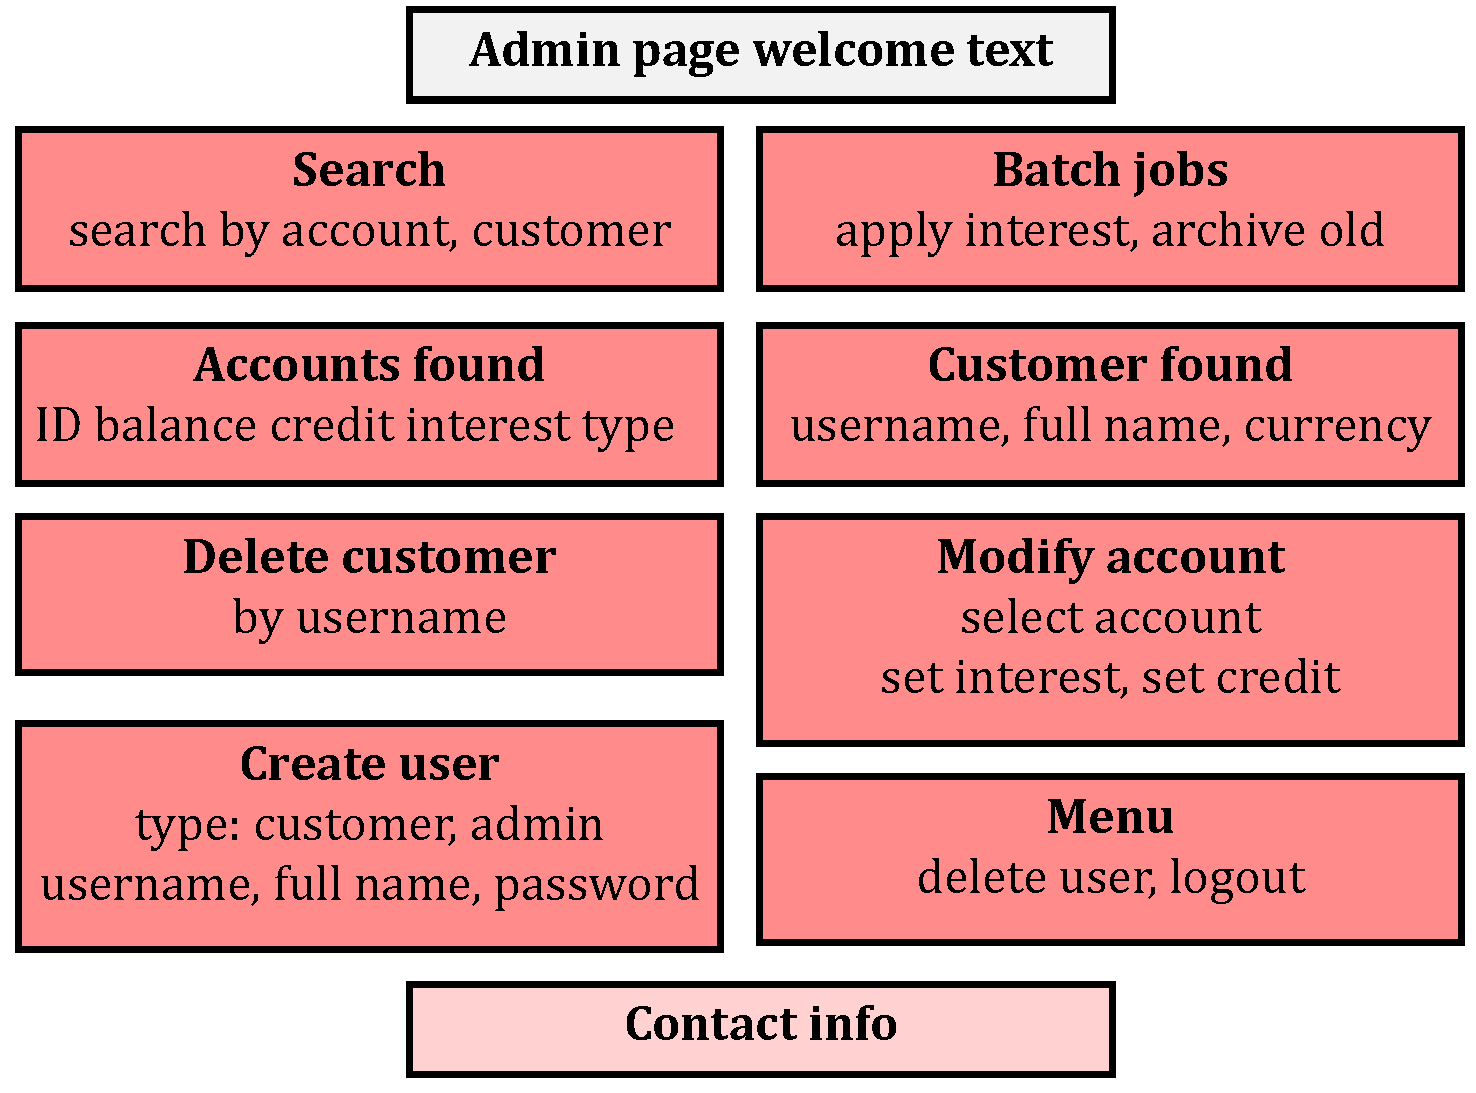
\includegraphics[width=\textwidth]{figures/adminPage.pdf}
\caption{Intended content in the admin page.}
\label{fig:adminPageDesign}
\end{subfigure}

\caption{View design: intended content in the two user pages.}
\end{figure}

\textbf{Dividing users:} Initially we considered just having a single user page. Upon login, the application should decide which buttons and actions should be accessible and shown. But as the project progressed, the divide between customer actions (e.g. transfer money) and admin actions (e.g. search) became prominent, so we divided the user page into two separate pages: customer page and admin page. The intended contents in the customer page and admin page are seen in Figs \ref{fig:customerPageDesign} and \ref{fig:adminPageDesign}. Account information should be shown as text, possibly through a \texttt{toString} method in an Account object.

\textbf{Errors:} When a user performs an illegal action, an error message should be shown to the user. This functionality can be integrated into Java exceptions, but should be displayed by View classes.
\subsection{Controller design (Mikkel)}

Since the program has several different components that must communicate, it was important for us to have these communications centralized as much as possible. This resulted in having three controllers throughout the program. These correspond to the three main parts, namely the user interface, the internal logic and the database. Since we have a singular controller for each of these, it is very easy to extend the functionality of the program as a whole. 

% Needs more.... very not finished

\begin{figure}[H]
\centering
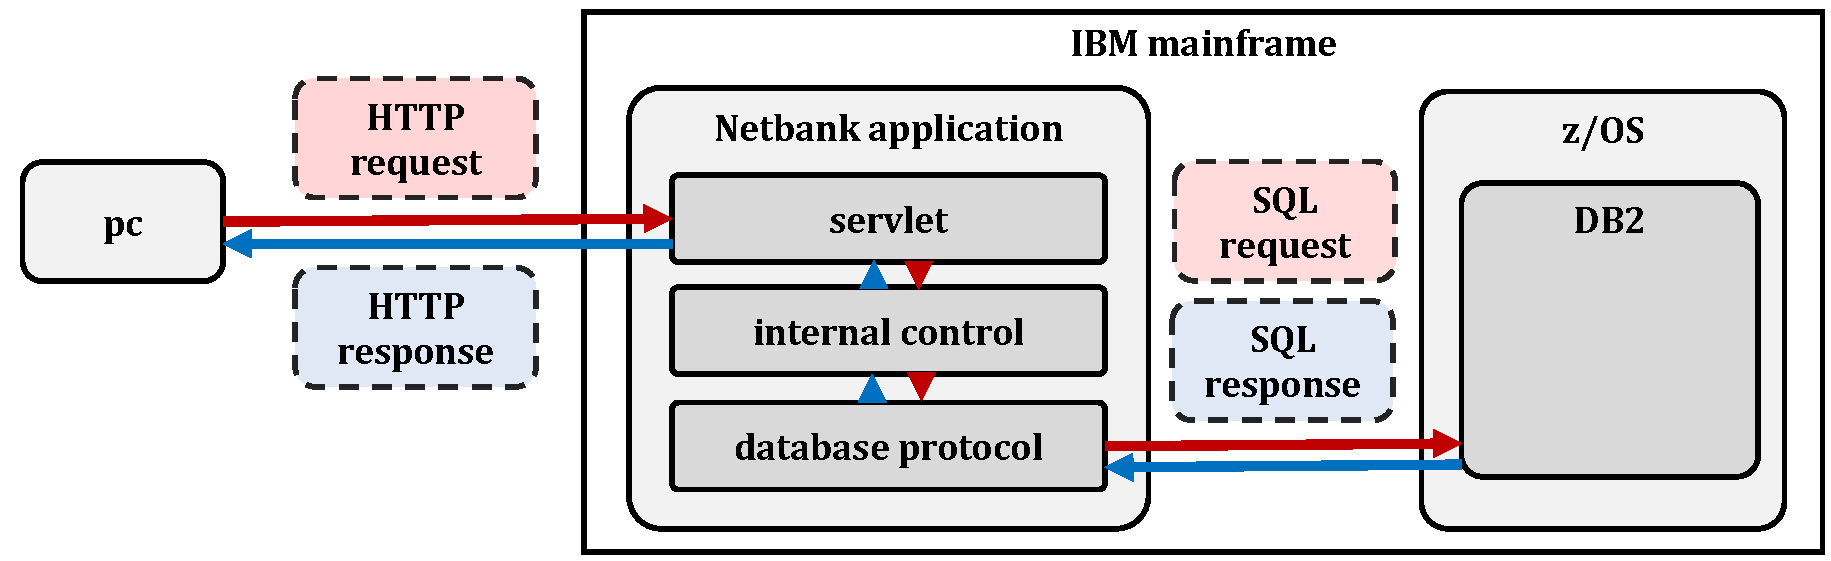
\includegraphics[width = 0.9\textwidth]{figures/control_flow.pdf}
\caption{Control flow in the program, and how the three controllers interact with the program.}
\label{fig:designcontrol}
\end{figure}
\subsection{Security design (Roar)} 
\label{sec:securitydesign}

When developing applications, and web applications in particular, it is of most importance that the application is secure. Securing an application is not a simple task, and is comprised of several aspects. We focused on the following:

\textbf{Passwords} should not be shown during the login, and encrypted when stored, ensuring that if a data leak of usernames and encrypted passwords should occur, it would be difficult to gain access to the accounts.

\textbf{Input sanitation} should be enforced, making sure that the application behaves as expected. Managing all input such as search tokens for SQL queries, and transfer amounts.

\textbf{Authority levels} are needed to differentiate between what customers and managing partners (admins) are able to do/see. 

\textbf{URLs} should not show confidential information or let other customers gain access to an account by entering the URL directly without logging in.

\textbf{Database} errors must be contained, keeping data uncompromised. It must be possible to regain the data from before the error occurred. 

When implementing the application, these precautions must be kept in mind, to make the application as robust as possible. In case of an action which violates one of these security aspects (or other illegal actions) an appropriate error message should be given to the user, letting the user know that the action was not performed.
%% DESIGN SECTION END

%% IMPLEMENTATION SECTION START
\newpage
\section{Implementation}
%\subsection{Intro (0.1 p)}

In this section, we document how we implemented the design from the previous section. In addition, in each subsection the implementation choices are discussed. 
\subsection{Model implementation (Jens Carl)}
The application model consists of the classes shown in figure \ref{fig:MVC_CD}. When a customer or admin logs into the application, a corresponding \texttt{User} sub-class object is instantiated. From the database, the logged-in user's credentials are found and put into the object. This object is then set in focus as the user currently logged in, e.g. \texttt{customerLoggedIn}. Controllers modify and use methods from this object when the user performs actions in the application. After an action is complete, the fields in the object are stored in the same table row as where it was fetched from, for future use. In figure \ref{fig:dbTables} below, the structure of the database is illustrated and described. 

\begin{figure}[H]
    \centering
    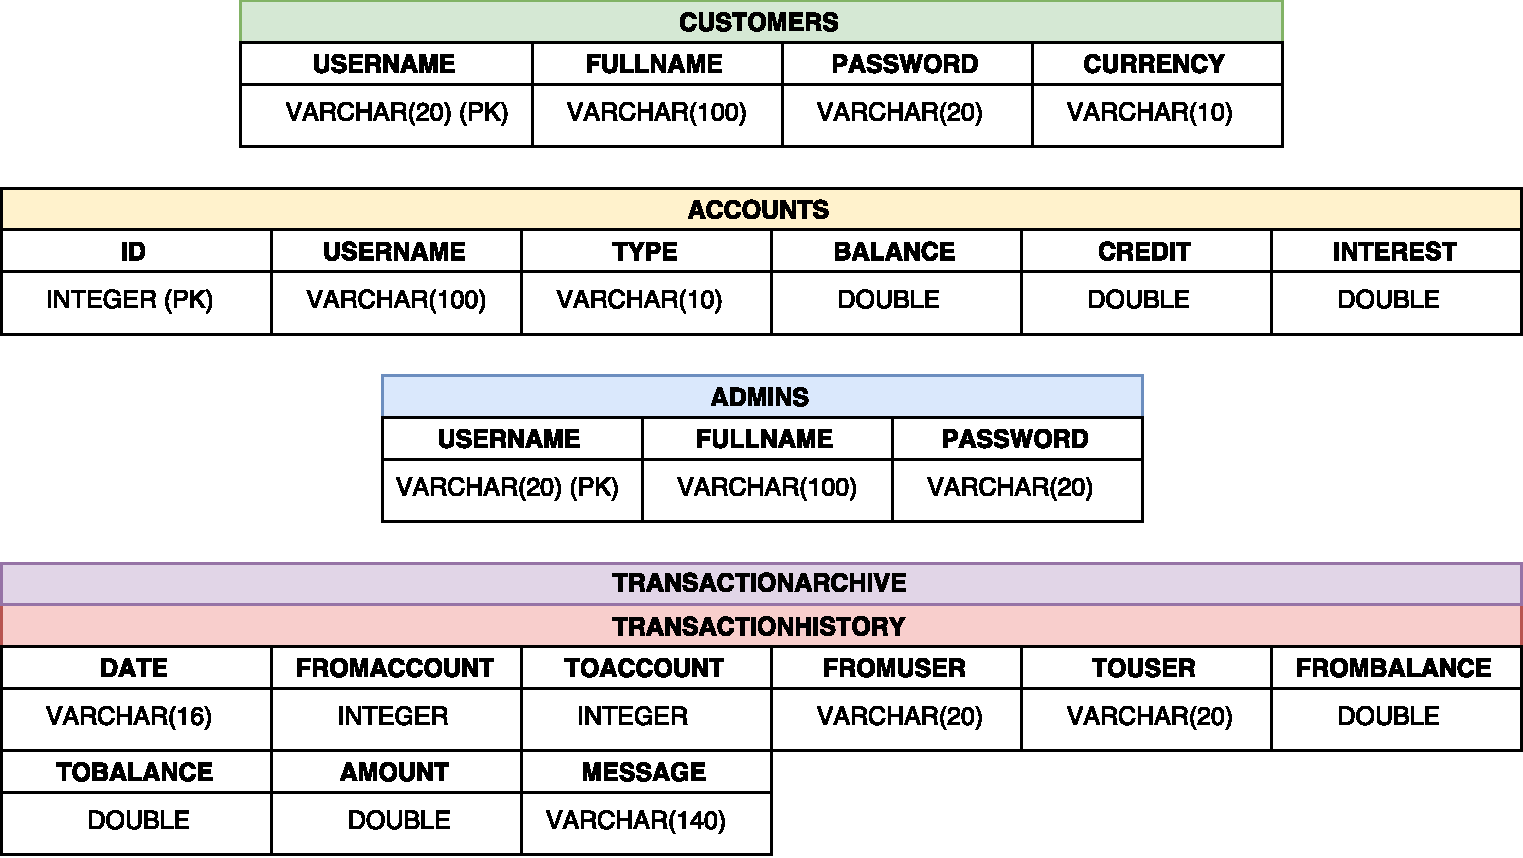
\includegraphics[width = 1.0\textwidth]{figures/dbTables.pdf}
    \caption{The table structure of the database was implemented to synergize with the operation procedure of the application. This means that, for example, the \texttt{ACCOUNTS}-table has roughly the same columns as fields in the \texttt{Account} java class. Likewise, this is true for tables \texttt{ADMINS} and \texttt{CUSTOMERS}, thus providing efficient and easy storage/fetching of required object constructor arguments for the application. 
    As the information required to store a transaction was spread across multiple Java objects, the table \texttt{TRANSACTIONHISTORY} was implemented otherwise. First we took a look at which elements we would like to store with a transaction, and then made a column for each of those. Later, a wrapper class \texttt{TransactionHistoryElement} was written in Java with fields equal to these columns. Table \texttt{TRANSACTIONARCHIVE} was created as a destination for migrating old transactions when performing batch jobs. It therefore has the same columns as \texttt{TRANSACTIONHISTORY}. Sample images of the database tables viewed in Data Studio can be seen in appendix section \ref{sec:apendixTables}.}
    \label{fig:dbTables}
\end{figure}



\subsubsection{Transaction History tables}
For a while we implemented dynamically generated tables. Each user had his/hers own table containing transaction history for that specific user. Later, however, this part of the model was replaced with just a single \texttt{TRANSACTIONHISTORY}-table holding all transactions in the bank. While dynamically generating tables seemed to provide an intuitive overview of data, we found it had two major flaws which proved to a deal-breaker: 1) it slowed down various operations substantially 2) it provided a sense of uncertainty about the current structure of the database, since the specific number of tables at any given time couldn't be predicted with certainty. 
%tables: customer, admin, accounts \\
%possible alternatives (dynamic, many tables) \\
%SQL statements, auto commit
             
\subsection{View implementation (Magnus)}

\textbf{Overview of files:} Each page mentioned in the View design section (\ref{sec:viewDesign}) has a corresponding JSP file, so we have: \texttt{loginPage.jsp}, \texttt{createCustomerPage.jsp}, \texttt{customerPage.jsp}, \texttt{adminPage.jsp}.
Each JSP file supports interspersed CSS, HTML and Java code. The JSP files interact with the rest of the application classes through a Servlet \texttt{DefaultServlet.java} (described in the following Control section).

\textbf{Forms:} Every user interaction is defined through an HTML \texttt{form} element. A form is a piece of code that is tied to a button, drop-down menu or similar. When a button is clicked, the form parameters are sent through a \texttt{HttpServletRequest} object to the Servlet, signalling the user's actions.

\textbf{Boxes, blocks of code:} We chose to visually collect user actions into blue/red boxes (for figures, see Appendix \ref{sec:appendixView}). This lets the user know which actions are within the same domain. The external representation (what the user sees) reflects the internal code: For each box on a page with a set of user actions, there is a block of code (specifically a HTML \texttt{div} object) in a .jsp file with corresponding form elements. e.g. the "Edit account" box contains a drop-down menu for selecting accounts (form \#1), a "set as main account" button (form \#2), and a "delete account" button (form \#3). Boxes in \texttt{customerPage} are blue, boxes in \texttt{adminPage} are red.

\begin{figure}[H]
\centering
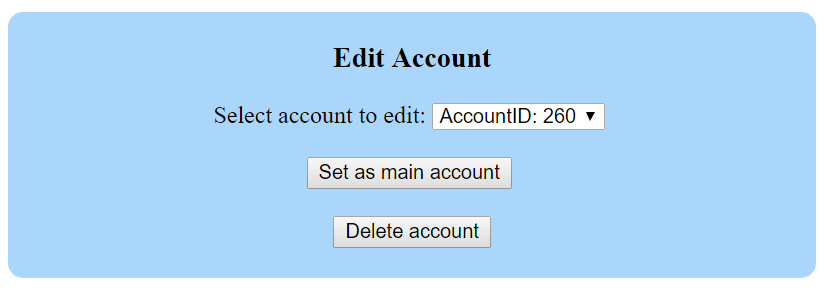
\includegraphics[width = 0.7\textwidth]{figures/forms.png}
\caption{Blue box "Edit account" in \texttt{customerPage.jsp}.}
\label{fig:forms}
\end{figure}

\textbf{HTML vs. toString:} 
When showing account information, we encountered a problem: the HTML code in jsp files ignores Java escape characters like \texttt{\textbackslash n} and \texttt{\textbackslash t}.
The solution was to  show account information in HTML tables instead. (see Fig \ref{fig:table_vs_toString}).


\textbf{Errors \& exceptions:} When a user performs an illegal action, a Java Exception is thrown internally. We implemented Exception subclasses with messages, and stored these messages in the \texttt{HttpServletRequest} object used by DefaultServlet. The error message is then displayed to the user in red text at the top of the web page. We considered using prompts, but personally found them too intrusive. How to display errors in an efficient but unobtrusive way is a subject well suited for testing.

\begin{figure}[H]
\centering
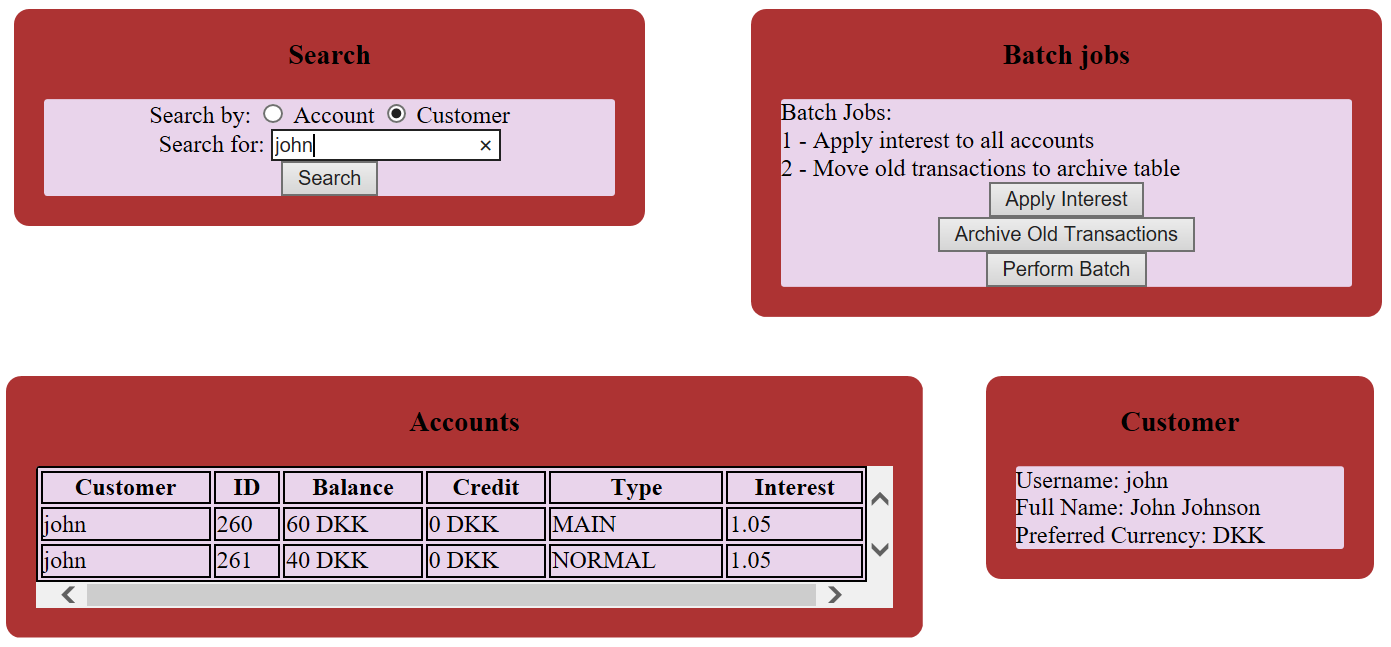
\includegraphics[width = 1.0\textwidth]{figures/adminPage_accounts.png}
\caption{An admin search for customer "john" through \texttt{adminPage.jsp}. Account information is shown in an HTML table instead of using a \texttt{toString} method. Searching by a customer by full name is not supported by the application.}
\label{fig:table_vs_toString}
\end{figure}

\subsection{Controller implementation (Mikkel) }
As mentioned in the Design section \ref{sec:securitydesign}, we divided the control into three classes, \texttt{BankApplication}, \texttt{DefaultServlet} and \texttt{DatabaseProtocol}. 

\begin{itemize}
    \item \texttt{BankApplication} handles the internal logic, comprised of Java code. Having a controller dedicated to the internal logic made it very easy to extend basic functionality throughout the coding process, and troubleshoot logical errors.
    \item \texttt{DefaultServlet} handles the webpages, and is thus a fairly simple controller. Its main responsibility is receiving HTTP requests, taking actions accordingly, and sending HTTP responses to the View pages.
    \item \texttt{DatabaseProtocol} handles the requests to the database and SQL statements.
\end{itemize}
  
The hierarchy between controllers goes as follows: \texttt{DefaultServlet} $\rightarrow$ \texttt{BankApplication} $\rightarrow$ \texttt{DatabaseProtocol}. This structure was chosen, as it corresponds with the way actions are carried out, starting through the interface $\rightarrow$ processed by internal logic $\rightarrow$ committing changes to the database. The control classes thus correspond to the different levels of abstraction, with the extremes being \texttt{DefautlServlet} knows what the user wants to do (but not how to do it) and \texttt{DatabaseProtocol} knows the data, but not what the user wants to do. This creates a structure where \texttt{DefaultServlet} is close to the View-part of the program, and \texttt{DatabaseProtocol} is close to the Model-part, more specifically the database. \texttt{BankApplication} acts as the bridge between the two, while also handling the Model-part of the program not in the database.

\begin{figure}[H]
\centering
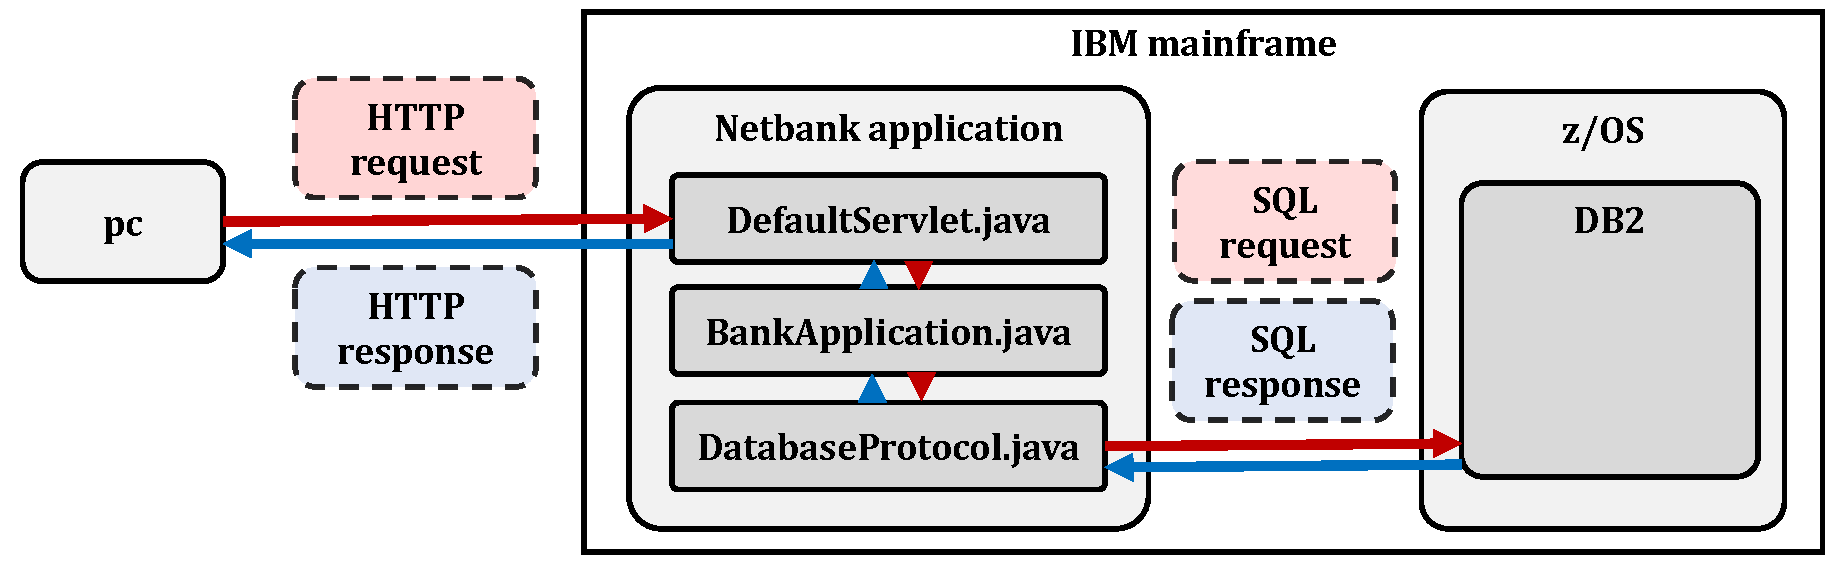
\includegraphics[width = 0.9\textwidth]{figures/interaction_transfer.pdf}
\caption{Control flow in the program, and how the three controllers interact with the program.}
\label{fig:interactiontransfer}
\end{figure}
\subsection{Security implementation (Roar)}

In order to integrate the security aspects as outlined in the design section \ref{sec:securitydesign}, several implementations are performed. 

\textbf{Hiding passwords} is done by using type "hidden" in the input form, in the loginPage.jsp page. 

\textbf{URL} data leak is avoided by sending the form to the main servlet's \texttt{post} method. This ensures that no field information is shown in the URL.

\textbf{Authority levels} are managed using a \texttt{User} class which is extended by a \texttt{Customer} and an \texttt{Admin} class. The different features are controlled by checking if the user is a customer or an admin. 

\textbf{Sanitizing input} is more complex. One of the simpler sanitizations is checking that transferred amounts only contains numbers, the value is positive, and the account has sufficient funds. Other sanitation implementations, are when a new customer is created; since usernames are kept unique and only comprised of lower case characters, this is ensured before creating the new customer. Another important input sanitation is when the user enters the username. Since this username is used in an SQL statement, SQL injections must be prevented. This is done using \texttt{PreparedStatement}, which distinguishes between executable SQL code and search tokens.

1The \textbf{database} connection is controlled in the highest control class \texttt{DefaultSevlet}, to make sure that all actions using the database are executed properly with the connection open. Maintaining the connection in the highest control class ensures that no deadlock is accidentally met, since all necessary database changes (requested from the user) are executed locally initially, and then committed as a whole, with the connections \texttt{autoCommit} feature set to false. If a database error occurs, it is then possible to rollback to the previous state of the data, since the changes are not yet committed. 
%% IMPLEMENTATION SECTION END

%% TEST SECTION START
\newpage
\section{Test}
 %\subsection{Intro (0.1 p)}
 
 In this section, we go over our test philosophy, present the 3 types of tests we considered, focusing on black box tests with JUnit and functional tests using participants.

\subsection{Test philosophy (Roar)}
 %Tests mainly used to create test-driven foundation for app class (core logic independent on database and view)
 
Automatic tests were used in the preliminary versions of the program, by JUnit tests. Since many features of the web program uses input from the View modules (user interface), testing becomes more involved. Back-end testing is preferred to validate the program below the presentation layer, in order to test the core of the program. We tested the core before it was integrating into a web application, which test the same features, but is easier to implement.
 
Other tests, like functionality tests were tested through the UI, and therefore performed in the later versions of the program. We could verify the results in database through Data Studio.
\subsection{Black box test (Mikkel)}

% \begin{mdframed}[backgroundcolor=black!5]
% funktionel test (ekstern test/black-box test) til at retfærdiggøre at
% ethvert krav fra kravspecifikationen er opfyldt (og at
% sammensætningen af de enkelte metoder virker efter
% hensigten).
%  \end{mdframed}
 
\subsubsection{Focus group}
In order to test the ease-of-use of our application, we wrote a list of tasks (see appendix \ref{tasklist}) a completely new user should be able to perform in 10 minutes or less without guidance. We then sent this to various users, garnering the following results.

\begin{table}[H]
    \centering
    \begin{tabular}{|c|c|c|} \hline 
        \textbf{Participants} & \textbf{Average time spent on tasks} & \textbf{Average age}\\ \hline
        7 & 6.8 minutes & 38.4 \\ \hline
    \end{tabular}
    \label{tab:focus_test_results}
\end{table}

%Non-technical focus group used our application, with focus on ease of use
As we can see, the average time spent on the tasklist is well below the estimated 10 minutes. This is a remarkable success, and we can confidently state that requirement nr. 12 has been fulfilled, even though the sample size was relatively small. 
 
\subsubsection{JUnit tests of application}
The JUnit tests were primarily used to ensure stability in the primary functions of the program. These correspond to actions such as creating users and accounts, as well as transferring money. As these are the actions users will mostly perform, it is important that they can be executed reliably. The tests primarily concern the same subjects as the ones on the task list we distributed for requirement 12, which can be seen in the appendix, section \ref{tasklist}.  

\subsection{Functionality tests (Mikkel)}
\label{sec:functionalitytests}
Since the program specifications mostly focus on user-interaction, the functionality tests are performed by hand, with program-level verification of correctness. As most of the program requirements are fairly easy to test by hand, we will here highlight some of the requirements that are a bit harder to test for a user, without switching between accounts.

\subsubsection{Performing batch-jobs}
Performing batch-jobs is done through the administrator page. The batch-jobs would normally only be performed once per week, but for testing purposes, we have not imposed a time limit.

A batch-job consists of two parts:
\begin{enumerate}
    \item applying interests to accounts
    \item moving old transactions to the transaction archive
\end{enumerate}
This complies with requirement nr. 10, although it goes a bit beyond, since the requirement only referred to moving elements in the transaction history. 

Pressing the \textit{"Perform batch"} button on the admin page starts the two aforementioned tasks. First, the rate of interest is applied to each account by pulling their current account balance, and multiplying it by the interest bound to it in the database. This can fairly easily be verified by searching for a user, performing a batch job, and noticing that their account balance increased. 

Archiving old transactions is a bit harder to verify, as transaction histories are only shown on a per-user basis on the customer page. In order to verify that archiving elements in the transaction history works, we need to look at the tables in the database, done through Data Studio. Since having a transaction that is a week old takes quite a bit of planning, we instead just perform a transaction and alter its date to be more than a week old. We then execute the batch-jobs from the admin page in order to move the transaction to the transaction archive table in the database. Going back into Data Studio, we can then see that the transaction has successfully been added to the \texttt{TRANSACTIONARCHIVE} table, and removed from the \texttt{TRANSACTIONHISTORY} table, thus verifying that the requirement has been fulfilled.

\subsubsection{Scalability}
For the purposes of this project, we were given a small partition of a database. This means that actually creating a million accounts is not possible, as we would simply run out of space, and thus testing requirement nr. 11 is not feasible. We can, however, comment on the scalability of our data structures. 

An example of how we have structured our program for scalability can be seen in how we store accounts in the database. The primary key of the \texttt{ACCOUNTS} table is represented by an auto-incrementing integer. This means that the number of accounts is only limited by the number of integers possible for the system, which is well above the required one million accounts. For the database as a whole, we have minimized the repetition of data between tables. Not only does this minimize the space we take on the partition as a whole, it also makes it so our application supports one user having a million accounts, as well as one million users having one account each. As the only part of our program affected by the total amount of data in the database are the SQL statements, and in extension the database itself, we can then conclude that our program can theoretically support one million accounts, as the IBM database allows for this, if not more.
\subsection{Performance test  (Magnus)}

We were asked by IBM not to performance test the application. The reason: we are 5 online bank groups, all running on the same z/OS partition on the mainframe. If one group crashes the partition, it affects all groups.\footnote{This actually happened June 13, when a group created 1 million accounts in their application, overloading the database.} But if we \textit{could} performance test our application, how would we do it? 

\textbf{Volume:} The application should be able to store 1 million accounts. This is actually a requirement in section \ref{sec:problemanalysis_requirements}, but we were asked not to test it. The accounts may be unevenly distributed. This can be tested by running a \texttt{for}-loop and creating 1-10 (randomly) accounts for 200 000 customers. This \texttt{for}-loop should be intentionally slowed, so it focuses on volume and not speed.  This may be achieved using the Java \texttt{sleep} method.

\textbf{Speed:}  The application should be able to manage a high number of transactions and logins per second. This can be tested by running a for loop with increasing size $N$ of simple transactions, until it crashes. 
For example: $N$ times, log in as A $\rightarrow$ send money to B $\rightarrow$ log in as B $\rightarrow$ send money to A. Print current $N$. For best results, we could use a computer cluster with many cores to bombard the application with requests.
%% TEST SECTION END

%% PROJECT MANAGEMENT START
\section{Project management and development}
\label{sec:projectmanagement}
%\subsection{Intro (0.1 p)}

In this section, describe how we organized, planned and carried out the project work in our group. Management and version control tools are presented and discussed.
\subsection{Organizing and planning (Roar)}

As a team, we have come to acknowledge the importance of organizing our workflow. At all meetings, a hearing is conducted involving a brief check-up of what was done last time, as well as what the next goals are. Once the goals are discussed and confirmed, the tasks are delegated. Depending on the tasks needed to be done, different approaches are used e.g. dividing up into subgroups or working as a whole. When implementing new features, it is more efficient to be divided up in smaller groups, to minimize code conflicts; while it is more efficient for everybody to work as a whole when larger design decisions are conducted. 

Often the working group (subgroup or whole) has a main programmer\footnote{This task often rotates, to keep one person from having full responsibility of coding.}, which implements the found solutions. The other member(s) confirm the solution and ensure that everything is covered.

To keep track of decisions, plans, schedules as well as assorted notes, we used a logbook. The logbook was kept in a shared text document. Here, we mostly wrote what we expected to work on at the start of the day as well as what we had finished by the end of the day, as conducted from the hearings. However, the logbook also contained possible features to implement, as well as several ideas on how to implement the different features. An excerpt from the logbook can be seen below.

\begin{figure}[H]
    \centering
    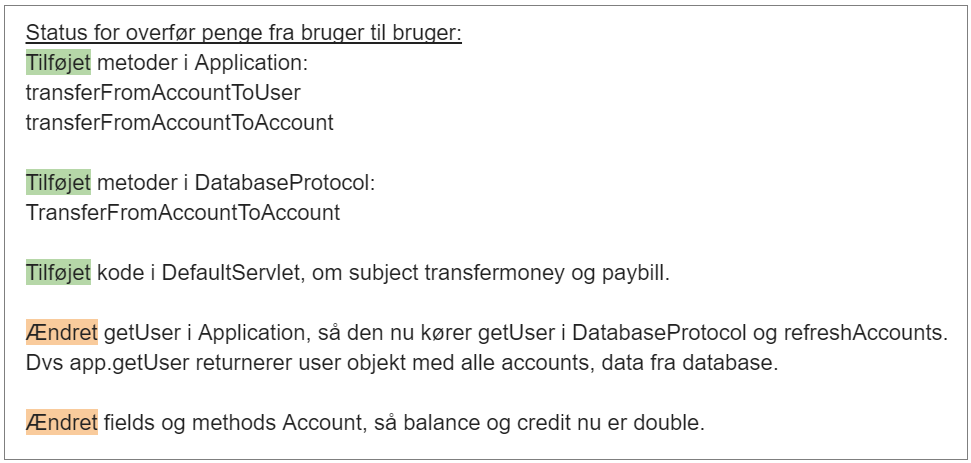
\includegraphics[width=0.7\textwidth]{figures/logbook2.PNG}
    \caption{An excerpt from the 30+ pages logbook. Application used: Google Docs.}
    \label{fig:logbook}
\end{figure}

\subsection{Git (Mikkel)}
We used Git as a the primary version control tool in order to have multiple groups of people implementing code simultaneously. As we primarily worked in pairs this meant we doubled our effectiveness by handling two problems at the same time. In order to achieve this, we had a routine of \textit{"Branch - Work - Merge"} once a day, if not more. One such occurrence can be seen in the figure below.

\begin{figure}[H]
    \centering
    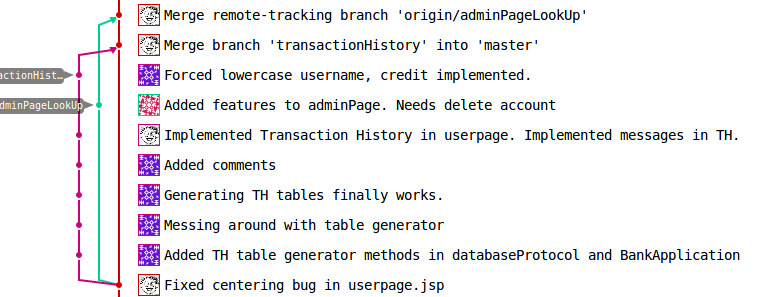
\includegraphics[width=\linewidth]{figures/git.png}
    \caption{An example of branching in the Git-commit timeline.}
    \label{fig:git}
\end{figure}


%how we used git. network figure, commit history figure.
\newpage
\subsection{Evolution of the program (Roar)}

The program was developed in four main steps. These steps are outlined in figure \ref{fig:PE}.

\begin{figure}[H]
    \centering
    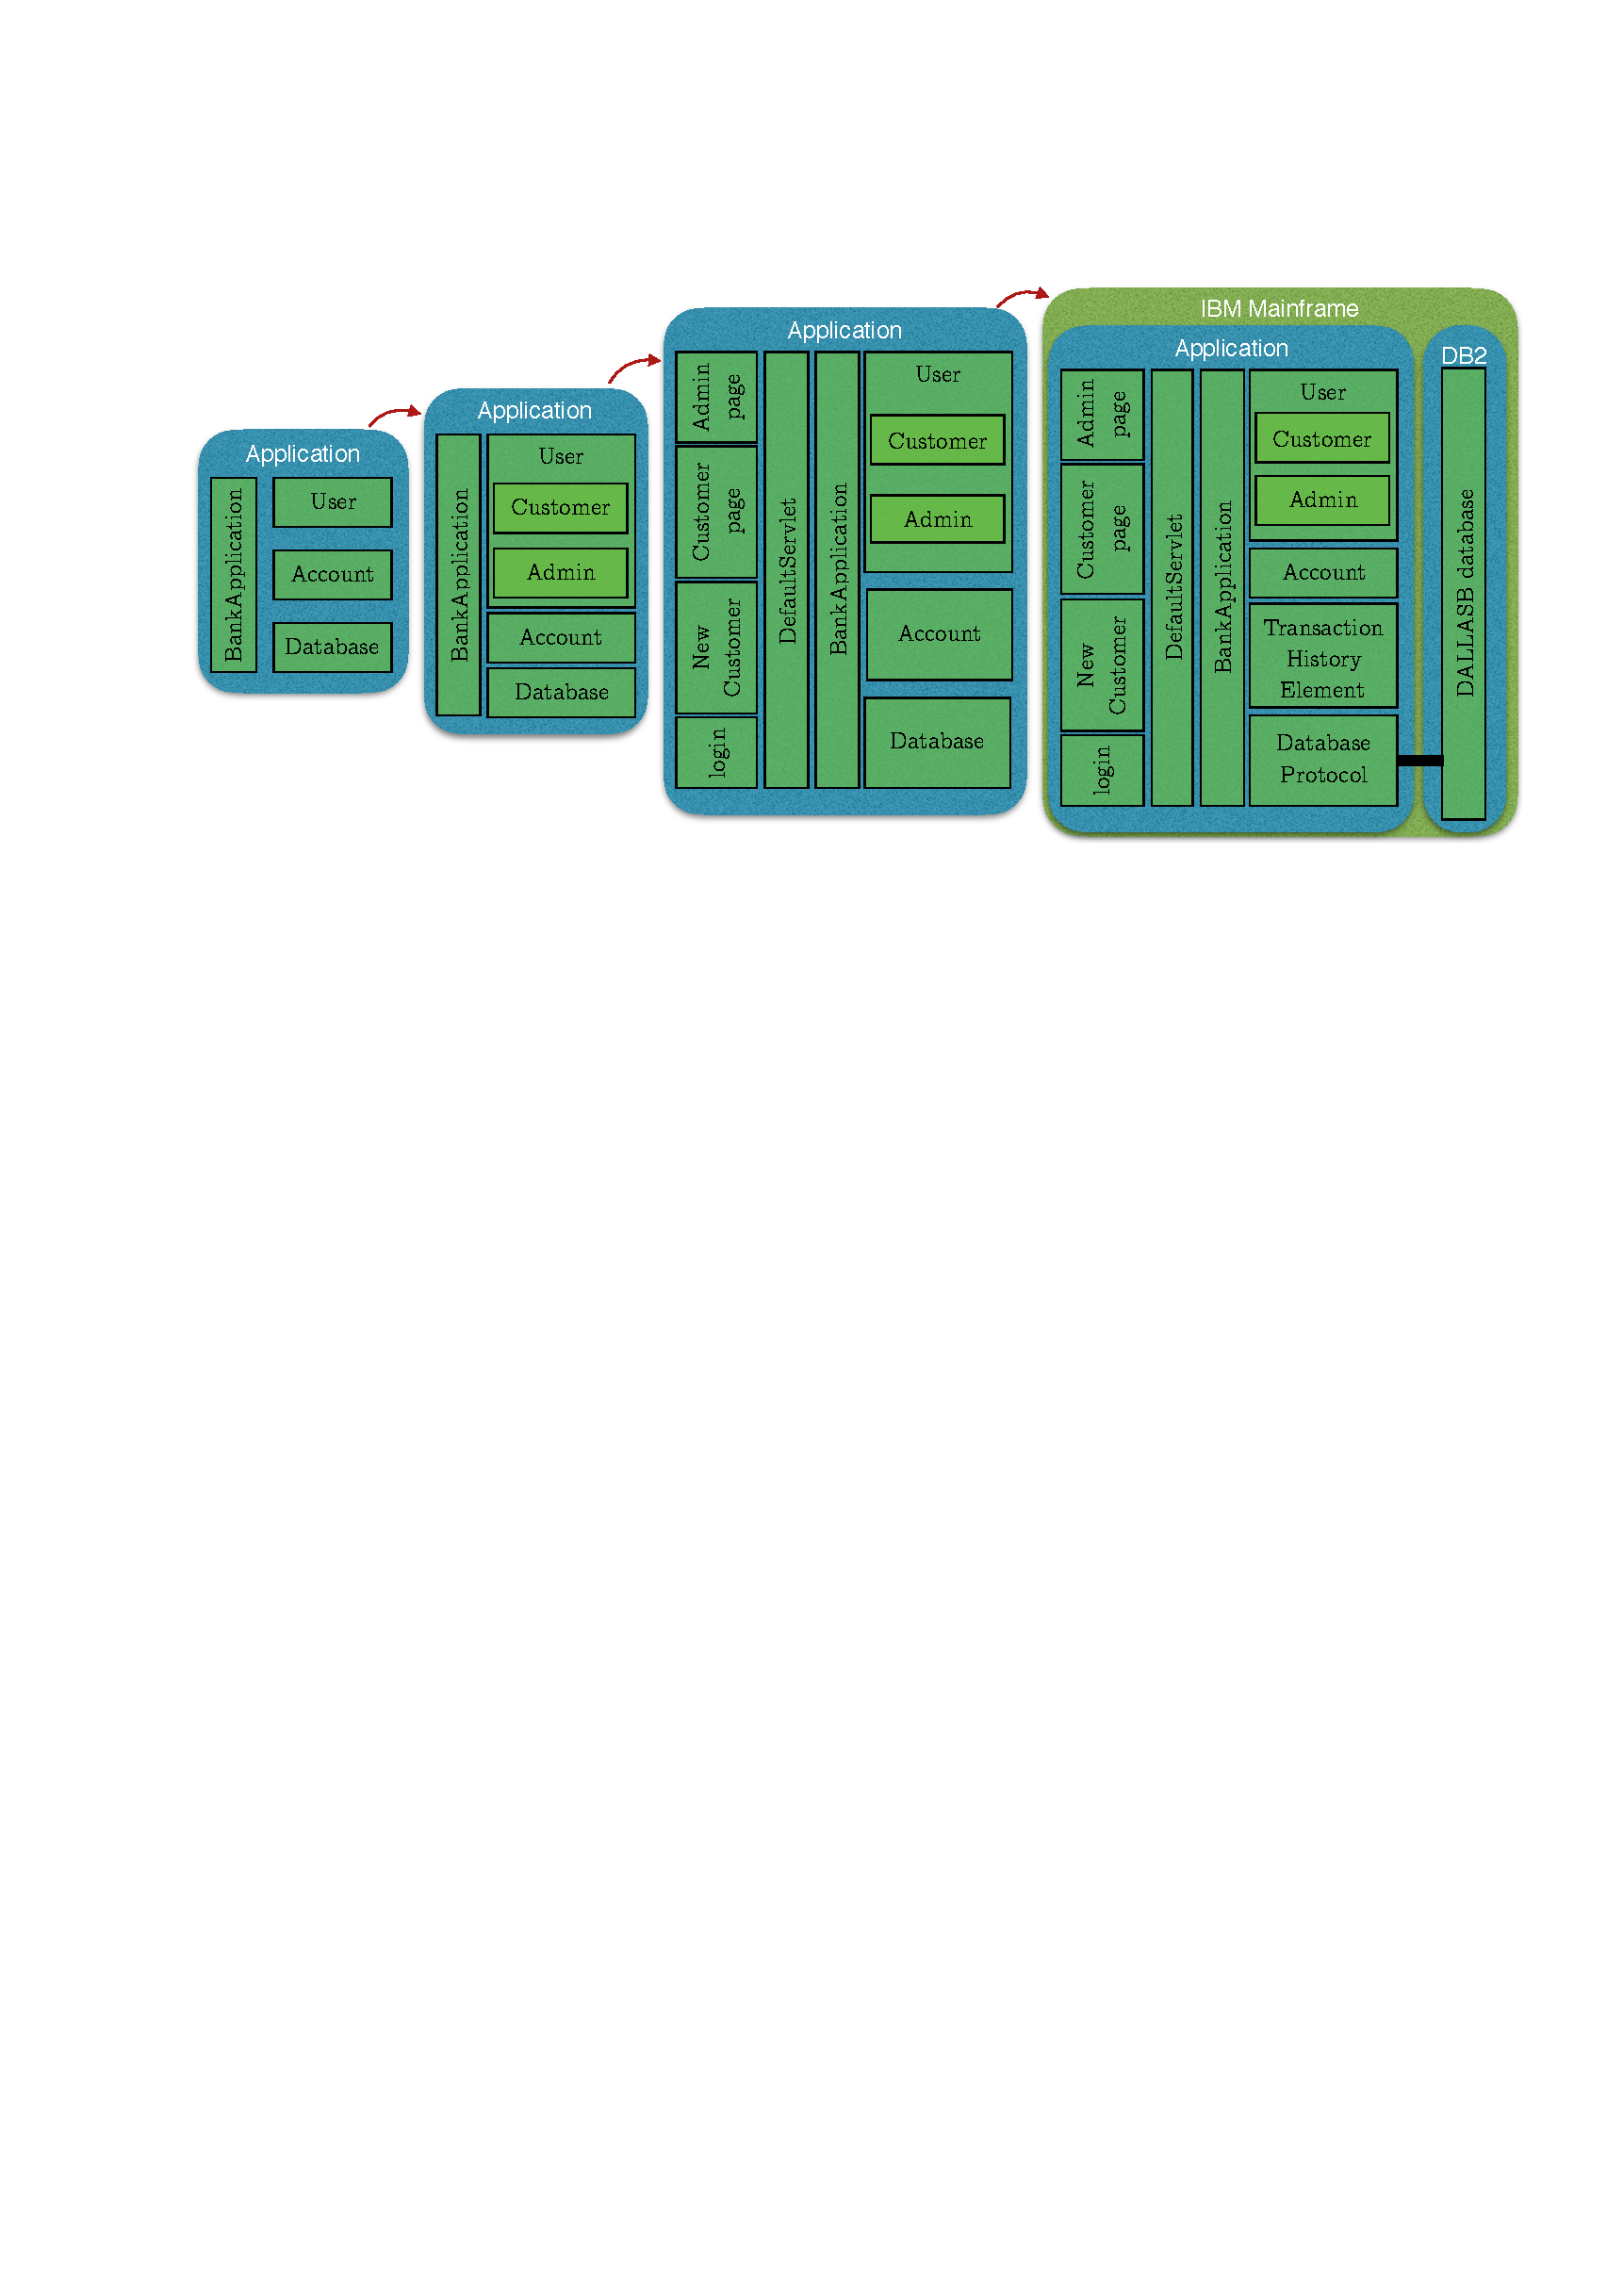
\includegraphics[width=\textwidth]{figures/PE}
    \caption{Outline of the four main stages of the program. At every stage the we had a fully working program, our development structure was inspired by agile development.}
    \label{fig:PE}
\end{figure}

\textbf{Stage 1:} At first, the program was comprised of the classes: \texttt{BankApplication}, \texttt{User}, \texttt{Account} and an auxiliary class called \texttt{Database}. These were implemented as the core of the program, with the \texttt{User} and \texttt{Account} as the model and \texttt{BankApplication} as the controller. The \texttt{Database} class's only purpose was to simulate the interaction with the database. No UI was created at this point, since the application was tested with direct method calls. Since the tools needed to connect the program with e.g. the database was not granted from the start of the course, this made it possible to encapsulate what the heart of the program was and test our ideas.

\textbf{Stage 2:} The next big step was to divide (or rather extend) the users into customers and admins. This made it possible to distinguish between customers and admins when features were allowed to one but not the other.

\textbf{Stage 3:} Then the application was made to run on a Java servlet, turning the application into a web application. The servlet was implemented in the \texttt{DefaultServer} class, and was the main link between the user and the application. \texttt{BankApplication}, whose main job is to alter the model, was not changed. Instead the \texttt{DefaultServer}'s job was made to convert the user input into the apropriate tasks for the \texttt{BankApplication} to carry out. With the DefaultServlet implemented, the next step was to create the UI from which the user interacts through. At first the UI was implemented through simple HTML files, but as more logic was needed in the separate pages, they all got converted into JSP files. This made them able to run Java code, as well as HTML and CSS code. 

\textbf{Stage 4:} When the database connection was implemented, the \texttt{Database} class was substituted with a class called \texttt{DatabaseProtocol}. This class contained the same features as the \texttt{Database} class, but instead of local storage in arrays, the data was stored in the DALLASB database delivered by IBM. Once the database was connected, the design of the program, was as planned, and has changed very little during the subsequent sessions. 

Besides the mentioned classes, some auxiliary classes were created. The exception classes help control the dataflow, when unwanted behavior is encountered. Also a wrapper class called \texttt{TransactionHistoryElement} for data transfer was written.
%% PROJECT MANAGEMENT END


\newpage
\section{Conclusion}
\subsection{Design (Jens Carl)}
\vspace{-0.2cm}
In sections \ref{sec:usecases} and \ref{sec:design}, use cases and tools were presented. The bank application was to be written in an object-oriented style using Java and make use of a DB2 database. With this in mind, a security level was designed including passwords, input sanitation, authority levels, hidden URLs and data storage stability. Model-view-controller was chosen as the architectural design pattern. This decision was primarily based on our team's previous experience and the scope of the project. All in all, designing from MVC proved to be successful as it was easy to design core features that corresponded to the specification requirements.  

% tools 
% object orienteed
% ibm
% security measures
% 
\subsection{Implementation (Roar)}

%conclusion on implementation. what was achieved? what can the app do?

The application was successfully implemented using the Model-View-Controller design pattern. The model is implemented as local classes with internal logic, as well as stored on a DB2 database for future access. The view is created using JSP files, only communicating with the controller through web forms. The controller is divided into three classes, each responsible for specific tasks in the MVC design. The controller manages all interaction between view inputs and the model. The application security is implemented with regards to hiding passwords, minimizing URL information, dividing authority, sanitizing inputs and handling database errors. The resulting implementation of the application satisfies the requirements outlined in section \ref{sec:problemanalysis_requirements}.
\subsection{Test (Mikkel)}

During the development progress, we used three types of tests. Early in the process, we used JUnit tests to ensure the stability of the core program. Later, when we had connected the database and finished all core features, we shifted to a 'usability' approach. Instead of testing the code directly, we tested features through the user interface. Finally, we showed our program to people who had not seen it before, and timed them going through a list of actions a user would commonly take. We then used their feedback and data to improve the ease-of-use of the program. We estimated a completely new user would be able to perform all tasks in the task list in 10 minutes or less, but ended up with an average time of 7 minutes. 

\subsection{Perspective (Magnus)}

The feedback from the test subjects in section \ref{sec:functionalitytests} provides a foundation for further development of our application. In particular, we would focus improvements on the following:
\begin{enumerate}
    \setlength\itemsep{-0.5em}
    \item Tooltips when hovering over buttons
    \item More intuitive error messages
    \item Support for several languages, changeable with a button
    \item Two-step authentication similar to NemID for increased security
\end{enumerate}

The technical experience we gained using the tools described in sections \ref{sec:ibm} and \ref{sec:tools} is easily transferable and to other DTU courses\footnote{such as 02170 Database Systems, 02267 Software Development of Web Services}, but more importantly: it is valued in the job market. 

Finally, the organizational experience described in section \ref{sec:projectmanagement} has brought us closer to being fully fledged software engineers able to systematically develop, evaluate and document larger software projects as a team.

\newpage
\begin{thebibliography}{9}

\bibitem{wikipedia_it_companies}
Wikipedia: List of the largest information technology companies \\
\url{https://en.wikipedia.org/wiki/List_of_the_largest_information_technology_companies}

\bibitem{fortune500}
Fortune 500: Technology sector\\
\url{http://fortune.com/global500/list/filtered?sector=Technology}

\bibitem{dtu_strategy}
DTU's strategy 2014-2019 \\
\url{http://www.dtu.dk/english/about/organization/strategy}

\bibitem{danmark_mest_digi}
version2: Danmark er det mest digitale EU land \\
\url{https://www.version2.dk/artikel/eu-undersoegelse-danmark-er-det-mest-digitaliserede-eu-land-104648}

\bibitem{digitalisering_oeger_produktivitet} Håndværksrådet: Digitalisering øger produktiviten \\
\url{https://hvr.dk/politik/h\%C3\%A5ndv\%C3\%A6rksr\%C3\%A5det-arbejder-for/digitalisering.aspx}

\bibitem{netbank_raadgiver}
business: Netbank er vigtiger end rådgiveren \\
\url{http://www.business.dk/bank/netbanken-er-vigtigere-end-raadgiveren-naar-vi-vaelger-bank}

\bibitem{netbank_foretrukken}
newsbreak: Netbank er blevet danskernes foretrukne bank \\
\url{http://newsbreak.dk/netbank-er-blevet-danskernes-foretrukne-bank/}

\bibitem{danskere_bruger_netbank}
Finanswatch: 88 \% af danskere bruger netbank \\
\url{http://finanswatch.dk/Finansnyt/Pengeinstitutter/article9113603.ece}

\bibitem{codd}
E. F. Codd: A Relational Model of Data for Large Shared Data Banks \\
\url{http://dl.acm.org/citation.cfm?doid=362384.362685}

\bibitem{db2}
db-engines: rankings of database systems \\
\url{https://db-engines.com/en/ranking}

\bibitem{danske_pengeinstitutter}
Wikipedia: Liste over danske pengeinstitutter efter størrelse \\
\url{https://da.wikipedia.org/wiki/Liste\_over\_danske\_pengeinstitutter\_efter\_st\%C3\%B8rrelse}

\bibitem{danskebank_java}
Danske Bank: Java is a new language on the mainframe\\
\url{https://www.youtube.com/watch?v=ACUUF2S9eGk}

\bibitem{html_most_used}
w3techs: Usage statistics and market share of HTML for websites \\
\url{https://w3techs.com/technologies/details/ml-html/all/all}

\bibitem{case_description}
DTU-IBM\_Mainframe\_Case\_2017.pdf

\bibitem{case_slides}
DTU Netbank Presentation 03022016 Final.ppt - Maria Kroos Boisen

\bibitem{ibm_history_slides}
History and evolution of IBM mainframes - Henrik Thorsen, IBM Technical Director

\bibitem{red_book}
Introduction to the New Mainframe: z/OS Basics (Third Edition) - Mike Ebbers, John Kettner, Wayne O’Brien, Bill Ogden

\end{thebibliography}

% \begin{mdframed}[backgroundcolor=black!5]
% Rapporten skal indeholde et afsnit med referencer til relevant materiale (bøger, artikler,
% rapporter, redskaber, som jeres arbejde på en eller anden måde bygger på)
%  \end{mdframed}

\newpage
%% APPENDIX START
\section{Appendix}
%
 
%  \begin{mdframed}[backgroundcolor=black!5]
%  User manual is often included as an appendix
% \end{mdframed}
\subsection{Glossary}\label{sec:glossary}

\begin{itemize}
    
    \item \textbf{Batch job:} A computer program (or set of programs) scheduled to run at a time where resources are easily available, e.g. a bank applying interest to accounts at night when few customers are using their web services.
    
    \item \textbf{CSS:} \textbf{C}ascasing \textbf{S}tyle \textbf{S}heets, a language used to set how a document (written in a markup language like HTML) is presented.
    
    \item \textbf{Database:} A storage place for data. In this context, the database is an IBM mainframe situated in Dallas, which was used to store table data.
    
    \item \textbf{DataStudio:} A program by IBM used to access and modify DB2 databases.

    \item \textbf{DB2:} Relational database system made by IBM.
    
    \item \textbf{HTML:} \textbf{H}yper\textbf{t}ext \textbf{M}arkup \textbf{L}anguage. The most popular markup language used for creating web pages and web applications.
    
    \item \textbf{HTML form:} Type of web form. Web forms allows user to enter data using checkboxes, radio buttons, or text fields. The data is then sent to a server and processed by a web application.
    
    \item \textbf{JavaScript:} A programming language commonly used in web-applications. Not to be confused with the programming language Java.
    
    \item \textbf{JSP:} \textbf{J}ava\textbf{S}erver \textbf{P}ages - a language which provides an easy way to integrate Java code into HTML files. Has the file extension \texttt{.jsp}, and compiles into Java servlets. In this context, they were used to generate servlets for the different pages in the application.
    
    \item \textbf{Mainframe:} A large computer that supports many workstations, and can run several partitions of operating systems. Focuses on robustness and up-time.
    
    \item \textbf{Netbank:} Short for inter\textbf{net} \textbf{bank}, a synonym for online bank.
    
    \item \textbf{PK:} Short for \textbf{P}rimary \textbf{K}ey.
    
    \item \textbf{RDBMS:} \textbf{R}elational \textbf{D}ata\textbf{b}ase \textbf{M}anagement \textbf{S}ystem, a database management system based on the relational model invented by IBM researcher E. F. Codd in the 1970s.

    \item \textbf{Servlet:} A type of Java program commonly used to integrate Java code into web-applications. The servlet itself has the file extension \texttt{.java}, but a servlet program can also be generated from JSP code, which has the file extension \texttt{.jsp}. 
    
    \item \textbf{SQL:} \textbf{S}tructured \textbf{Q}uery \textbf{L}anguage - the language used to send commands to the database tables in order to edit either the tables themselves or the data in them.
    
    \item \textbf{Sysplex:} Short for \textbf{sys}tem com\textbf{plex}. A sysplex is a cluster of IBM mainframes (or partitions on mainframes) acting as a single unit. Used to distribute workload, recover from disaster, and ensure high availability.
    
    \item \textbf{Table:} A collection of data in the database. Similar data will be stored in the same table, for example accounts are stored in an account table. Makes it easy to store and retrieve data whenever necessary.
    
    \item \textbf{Websphere Liberty:} A type of server, developed by IBM. %(IBM afsnit)
    
    \item \textbf{z/OS:} 64-bit operating system made for IBM mainframes.
        
\end{itemize}



\subsection{Task list (Mikkel)}
\label{tasklist}
\begin{enumerate}
    \item Create a new user
    \item Create a new account
    \item Send 5 money from your main account to your new account
    \item Send 5 money from your other account to the user \textit{magnus}, and attach a message
    \item Set the new account to be your main account
    \item Change your currency to EUR
    \item Delete an account 
    \item Log out from your user
\end{enumerate}

\subsection{View: Screenshots of pages (Magnus)}\label{sec:appendixView}

\begin{figure}[H]
\centering
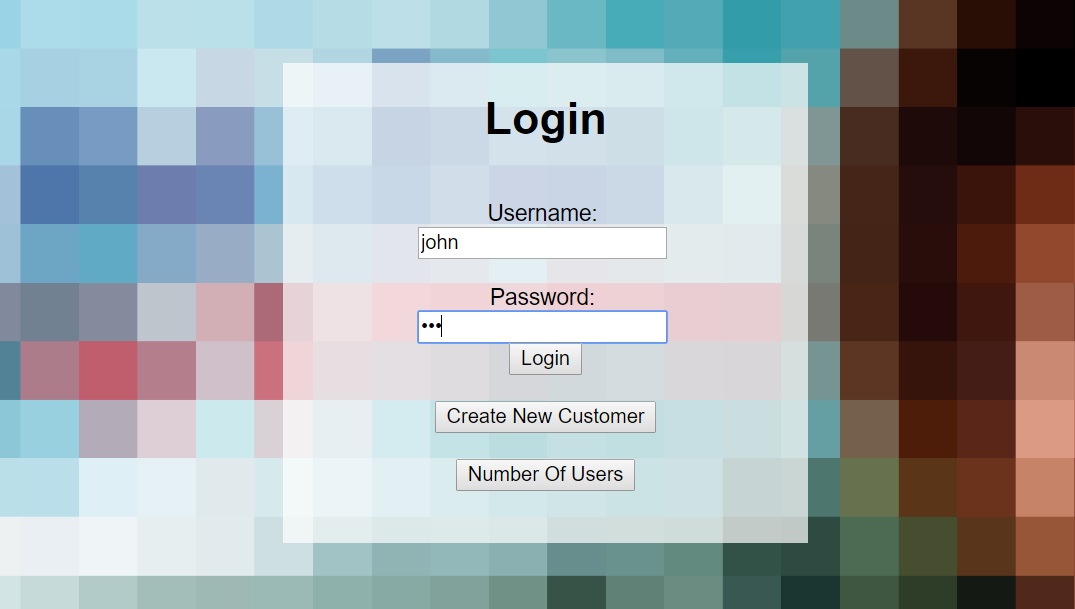
\includegraphics[width = 1.0\textwidth]{figures/loginPage.png}
\caption{Screenshot of the login page.}
\label{fig:loginPage1}
\end{figure}

\begin{figure}[H]
\centering
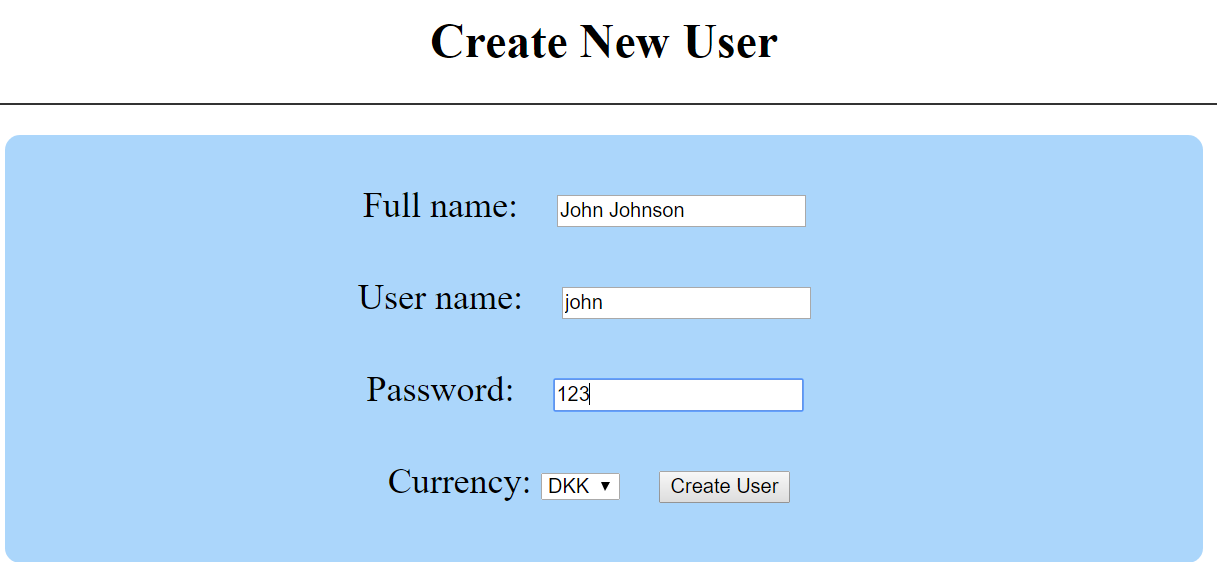
\includegraphics[width = 1.0\textwidth]{figures/newCustomerPage.PNG}
\caption{Screenshot of the new customer page.}
\label{fig:newCustomerPage2}
\end{figure}

\begin{figure}[H]
\centering
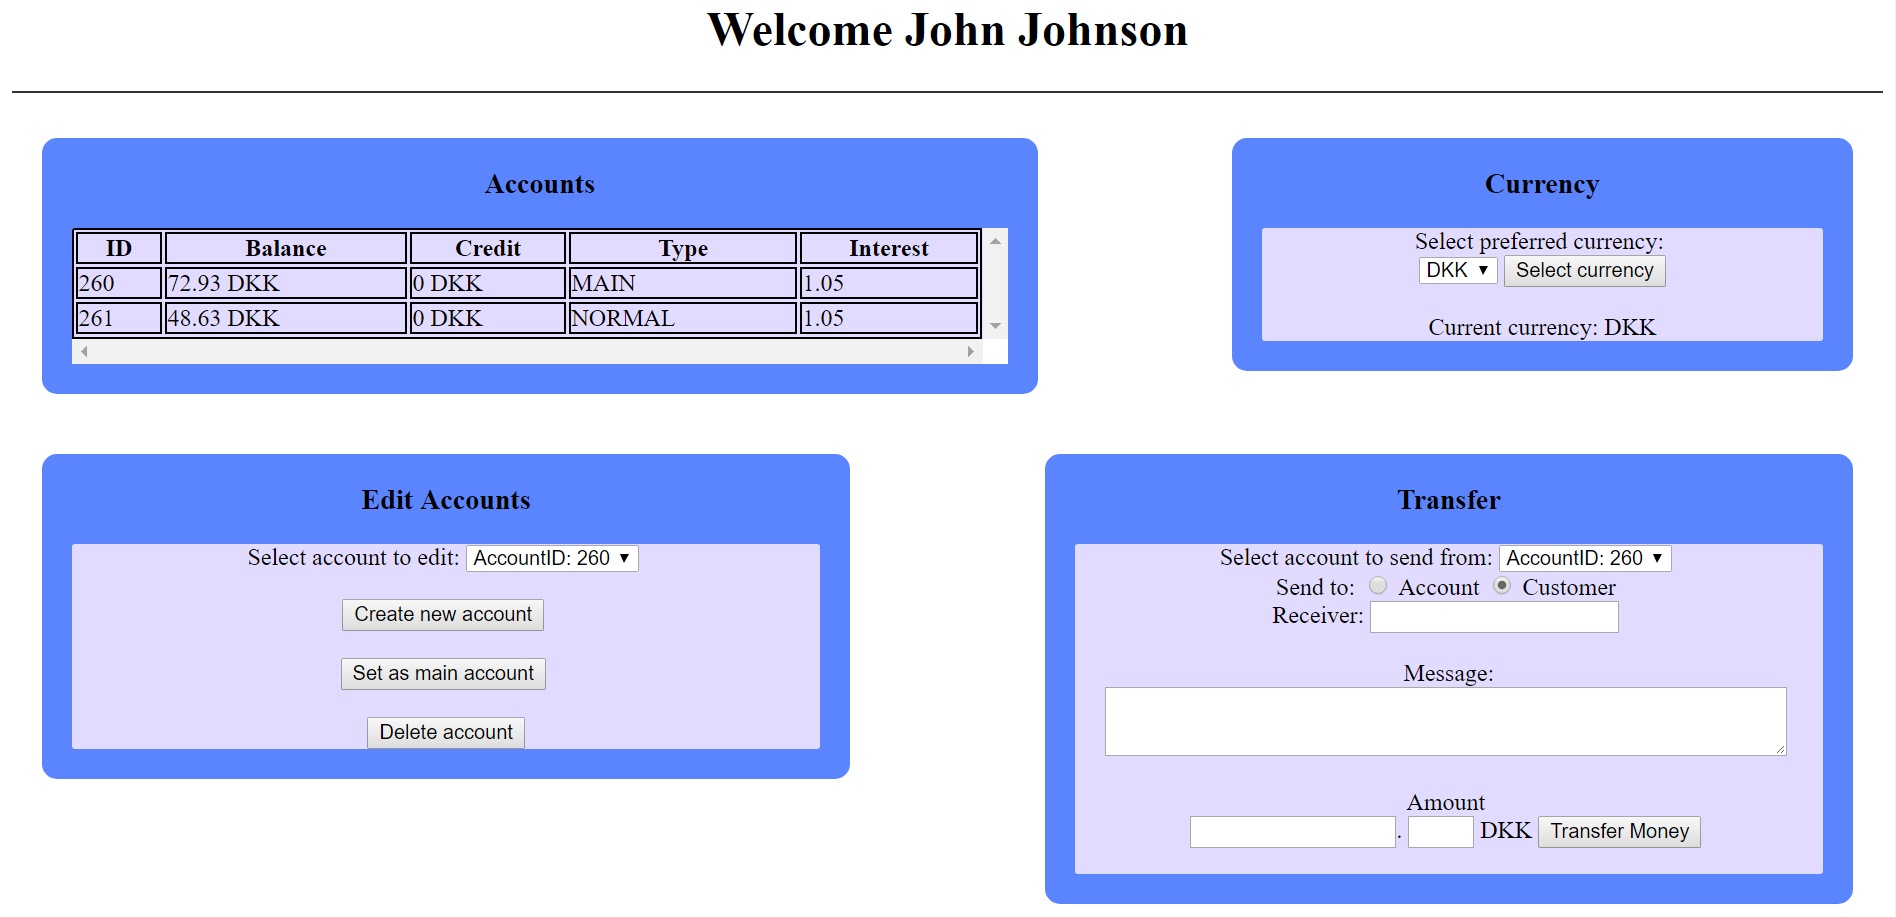
\includegraphics[width = 1.0\textwidth]{figures/customerPage1.png}
\caption{Screenshot of the customer page.}
\label{fig:customerPage1}
\end{figure}

\begin{figure}[H]
\centering
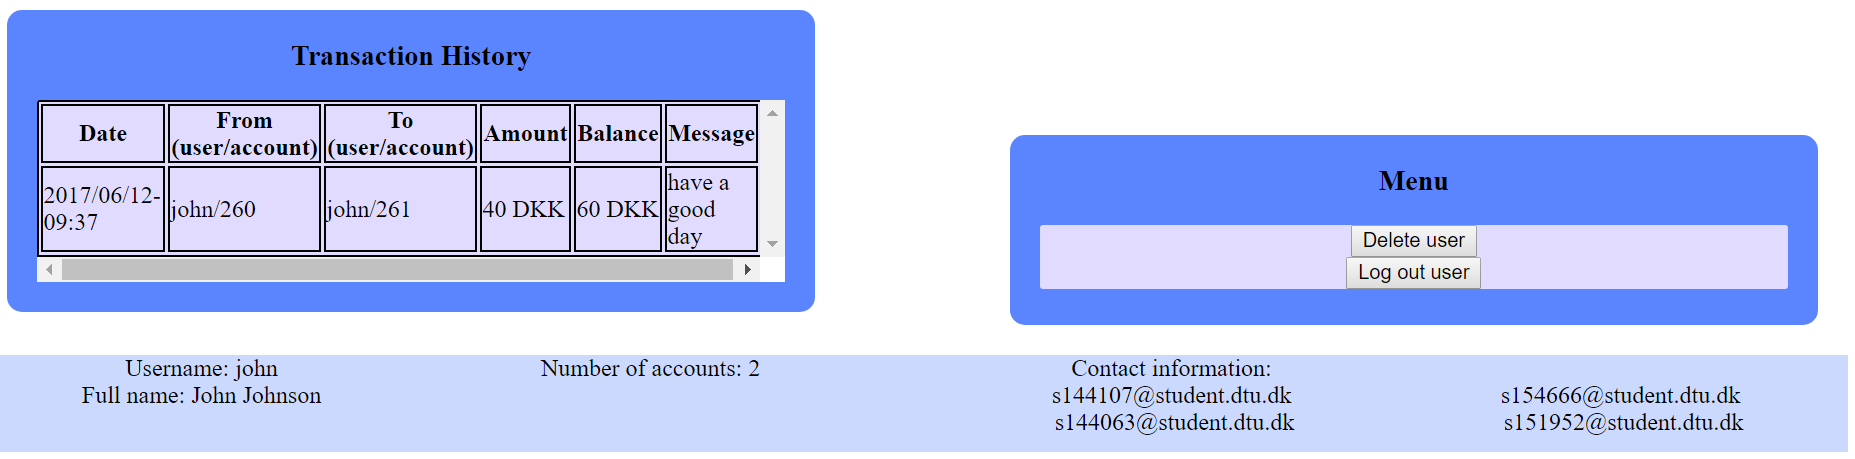
\includegraphics[width = 1.0\textwidth]{figures/customerPage2.png}
\caption{Screenshot of the customer page.}
\label{fig:customerPage2}
\end{figure}

\begin{figure}[H]
\centering
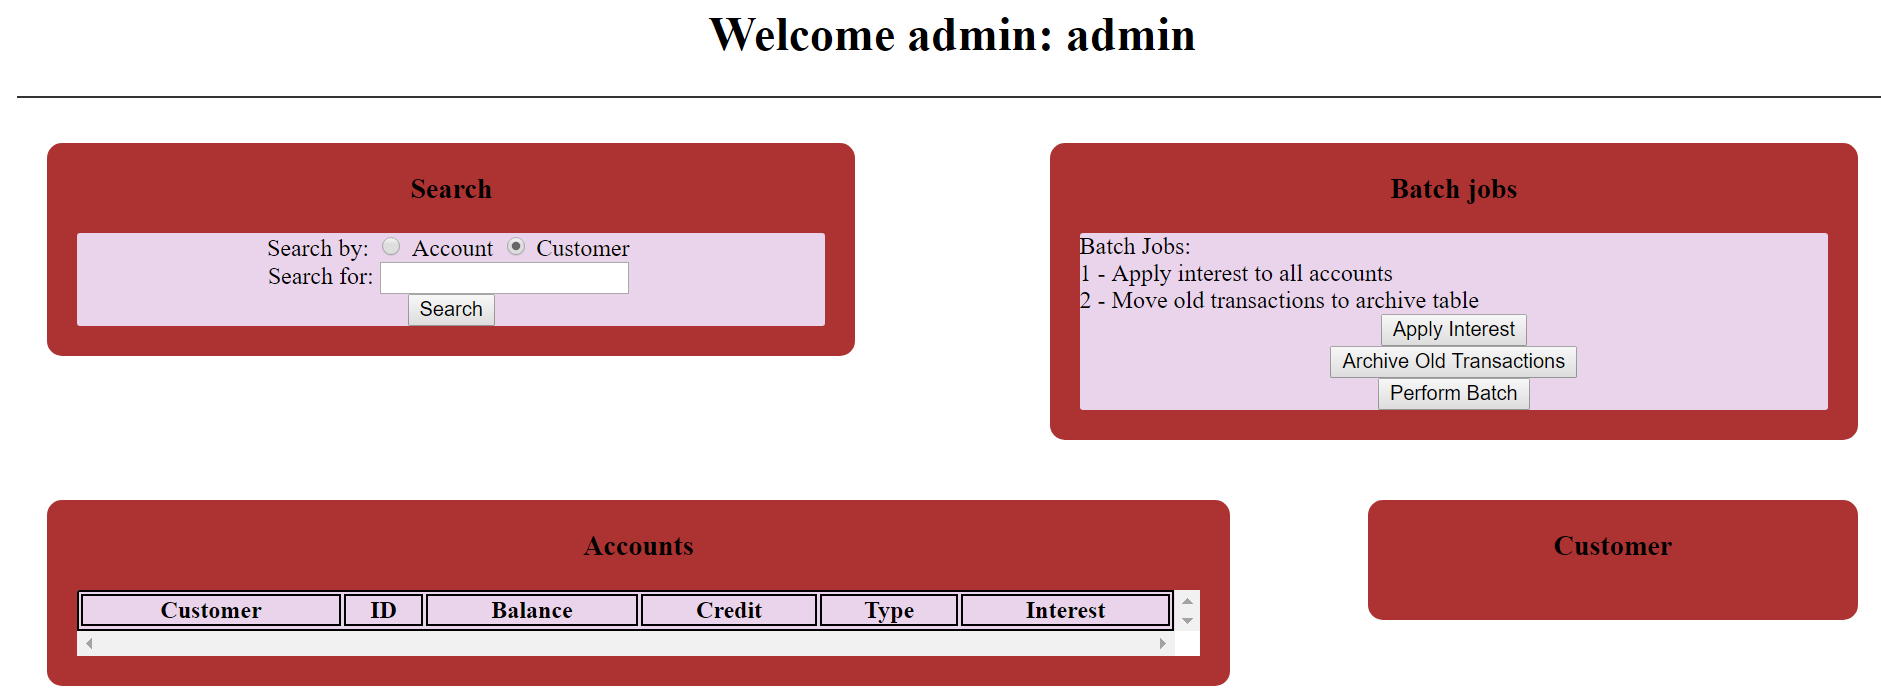
\includegraphics[width = 1.0\textwidth]{figures/adminPage1.png}
\caption{Screenshot of the admin page.}
\label{fig:adminPage1}
\end{figure}

\begin{figure}[H]
\centering
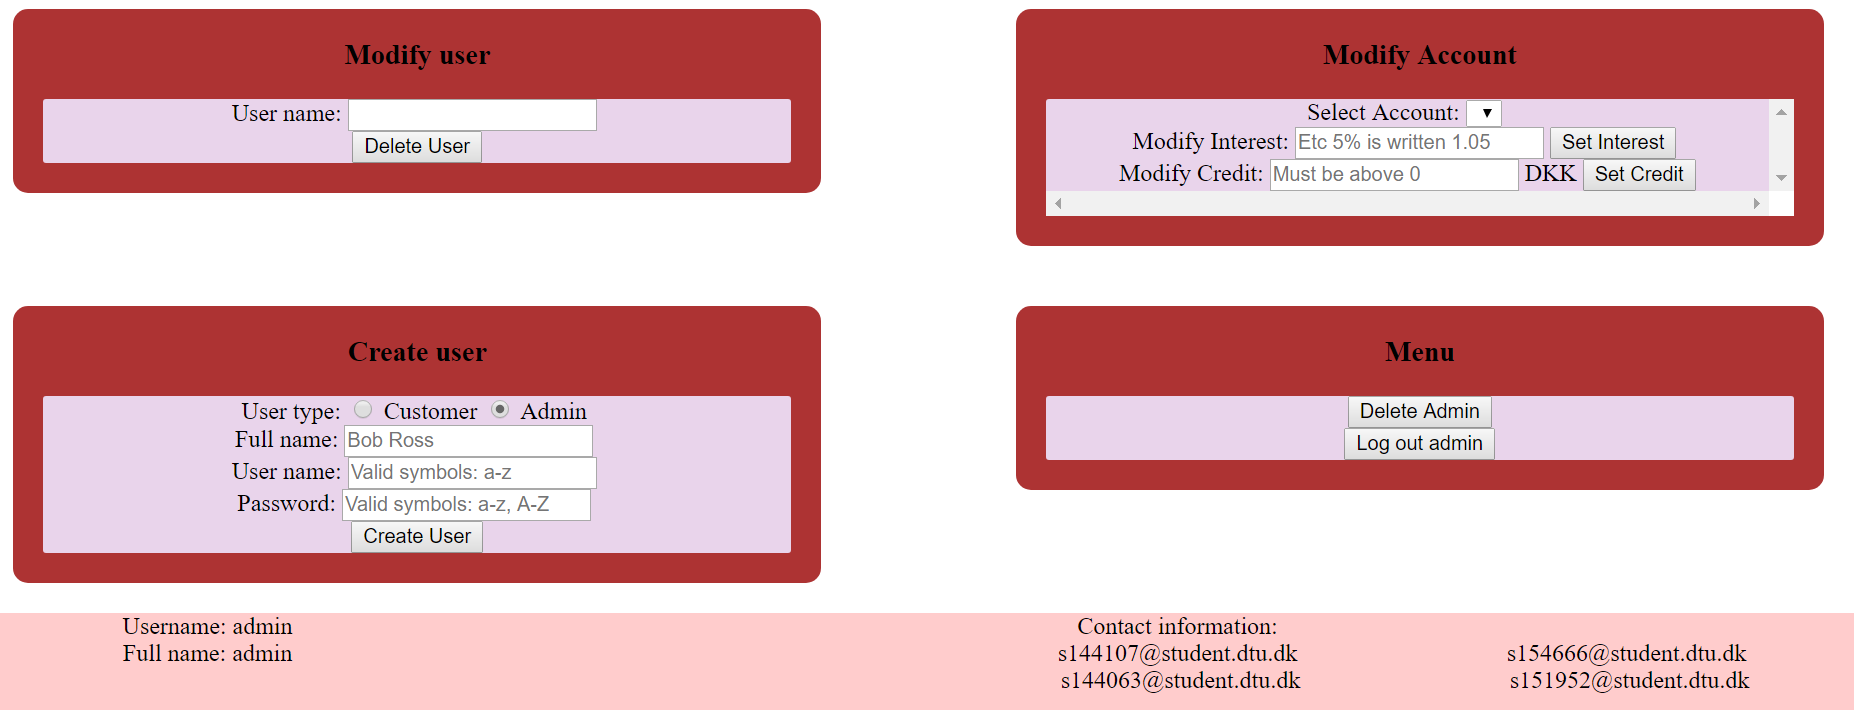
\includegraphics[width = 1.0\textwidth]{figures/adminPage2.png}
\caption{Screenshot of the admin page.}
\label{fig:adminPage2}
\end{figure}

\subsection{Database table sample images (Jens Carl)}\label{sec:apendixTables}
\begin{figure}[H]
    \centering
    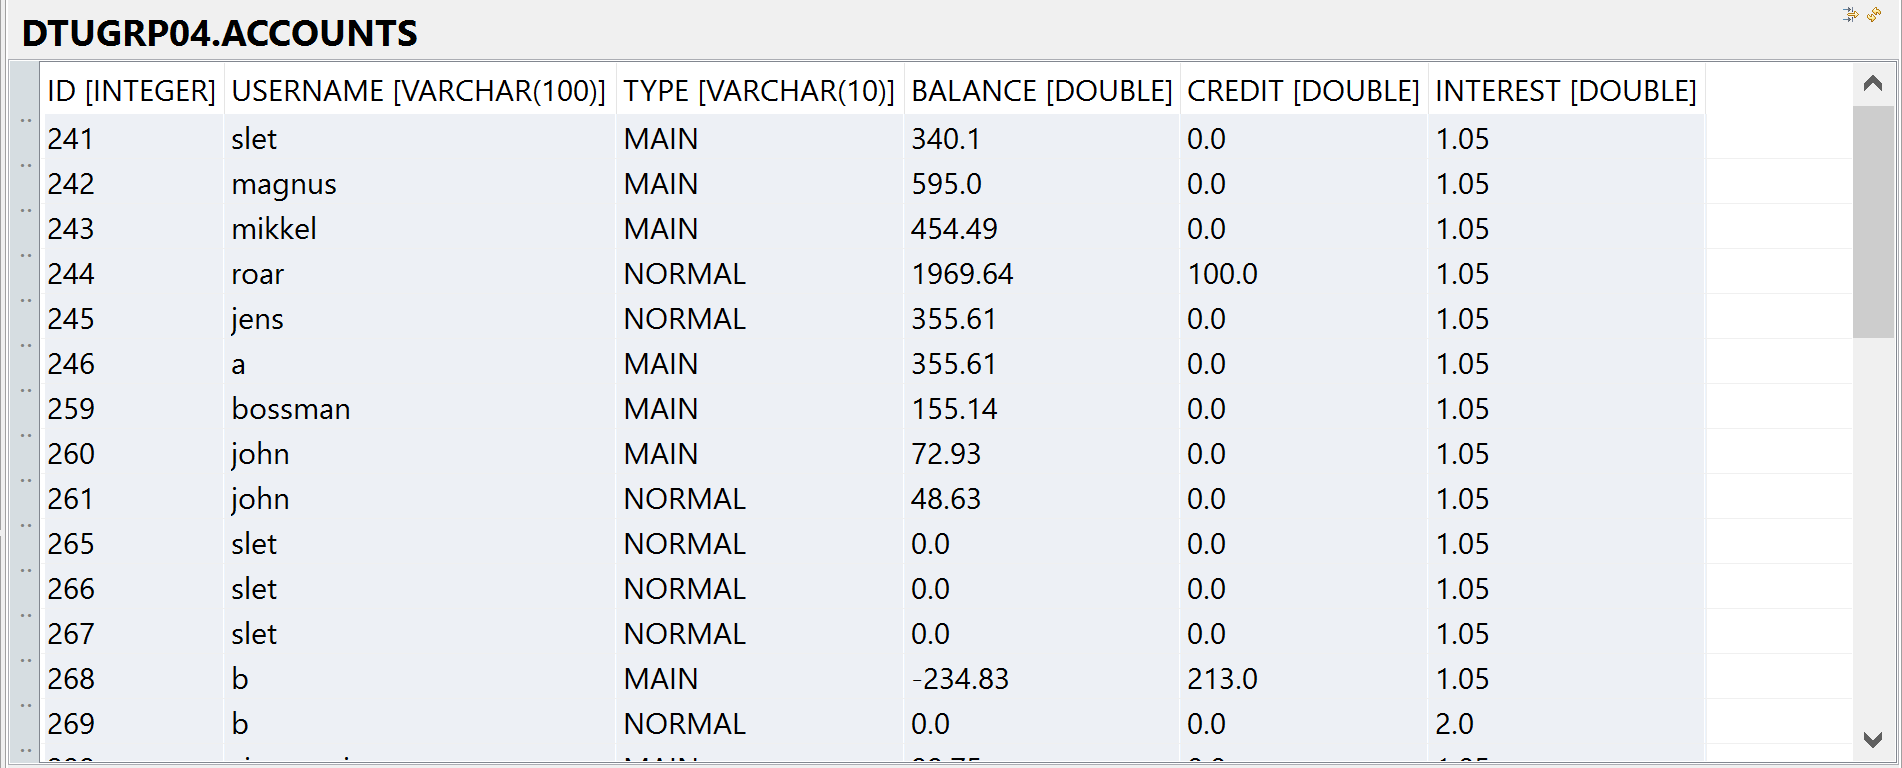
\includegraphics[width=\textwidth]{figures/accountsTable.PNG}
    \label{fig:accountsTable}
\end{figure}
\begin{figure}[H]
    \centering
    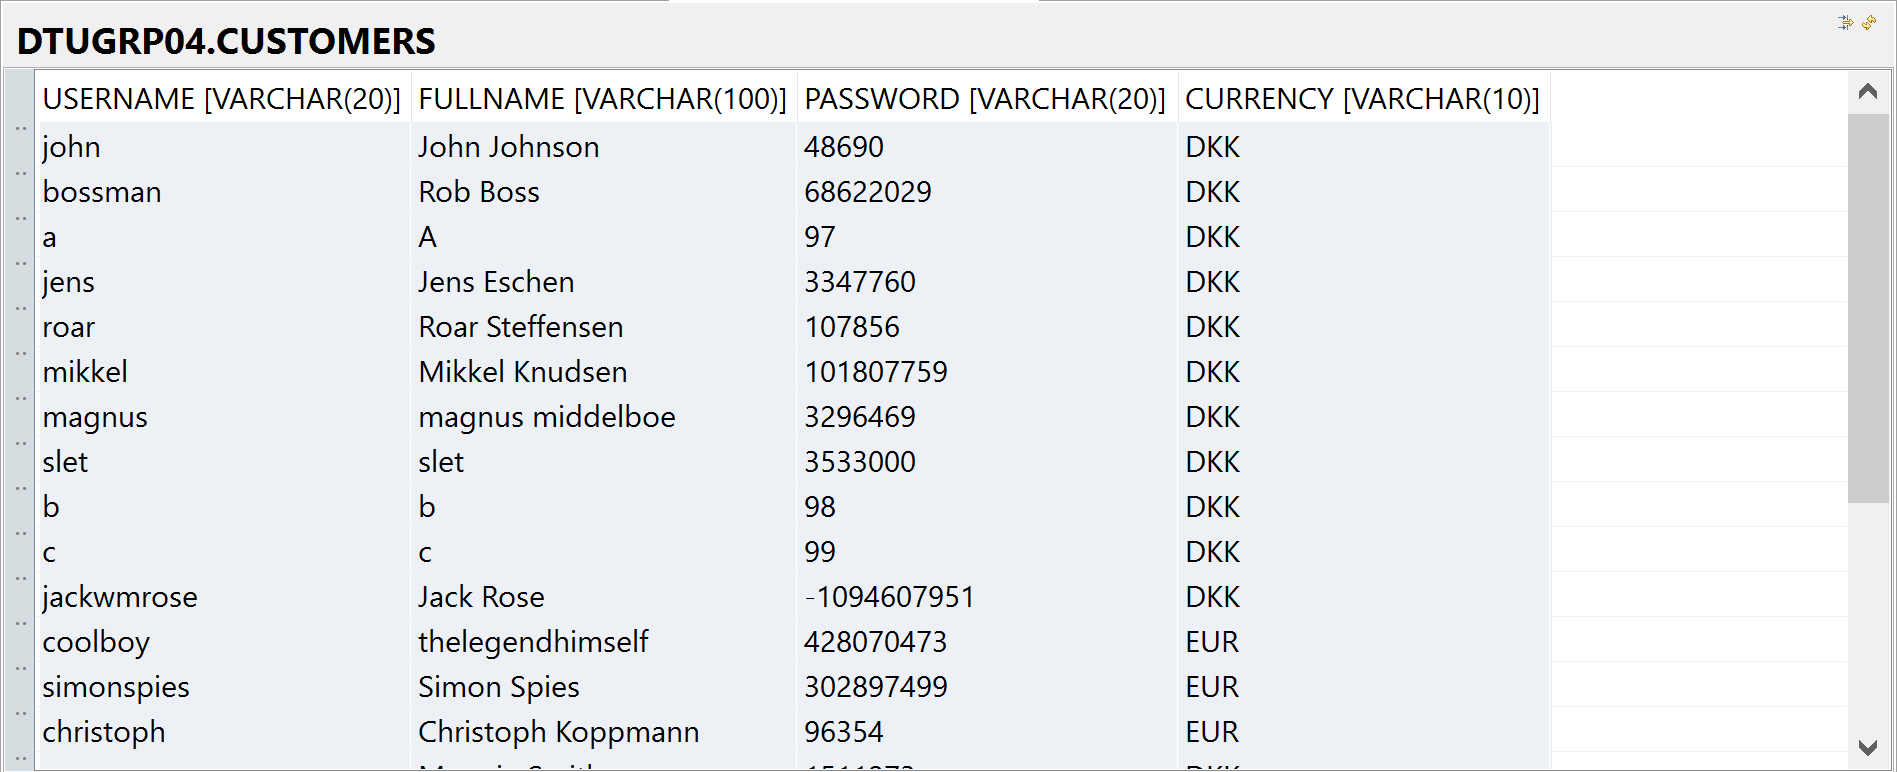
\includegraphics[width=\textwidth]{figures/customerTable.PNG}
    \label{fig:customersTable}
\end{figure}
\begin{figure}[H]
    \centering
    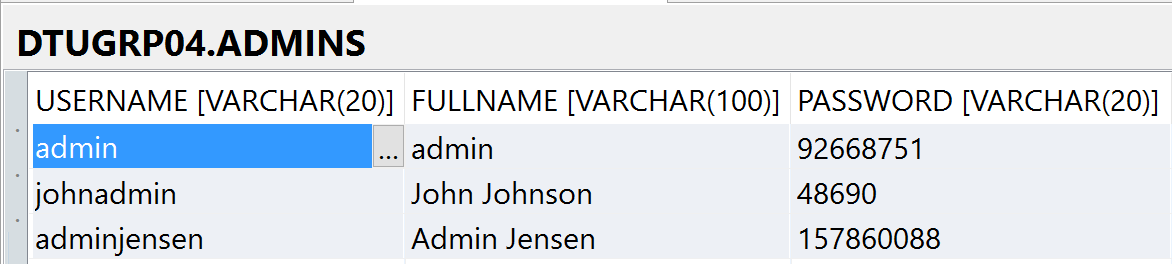
\includegraphics[width=\textwidth]{figures/adminsTable.PNG}
    \label{fig:adminsTable}
\end{figure}
\begin{figure}[H]
    \centering
    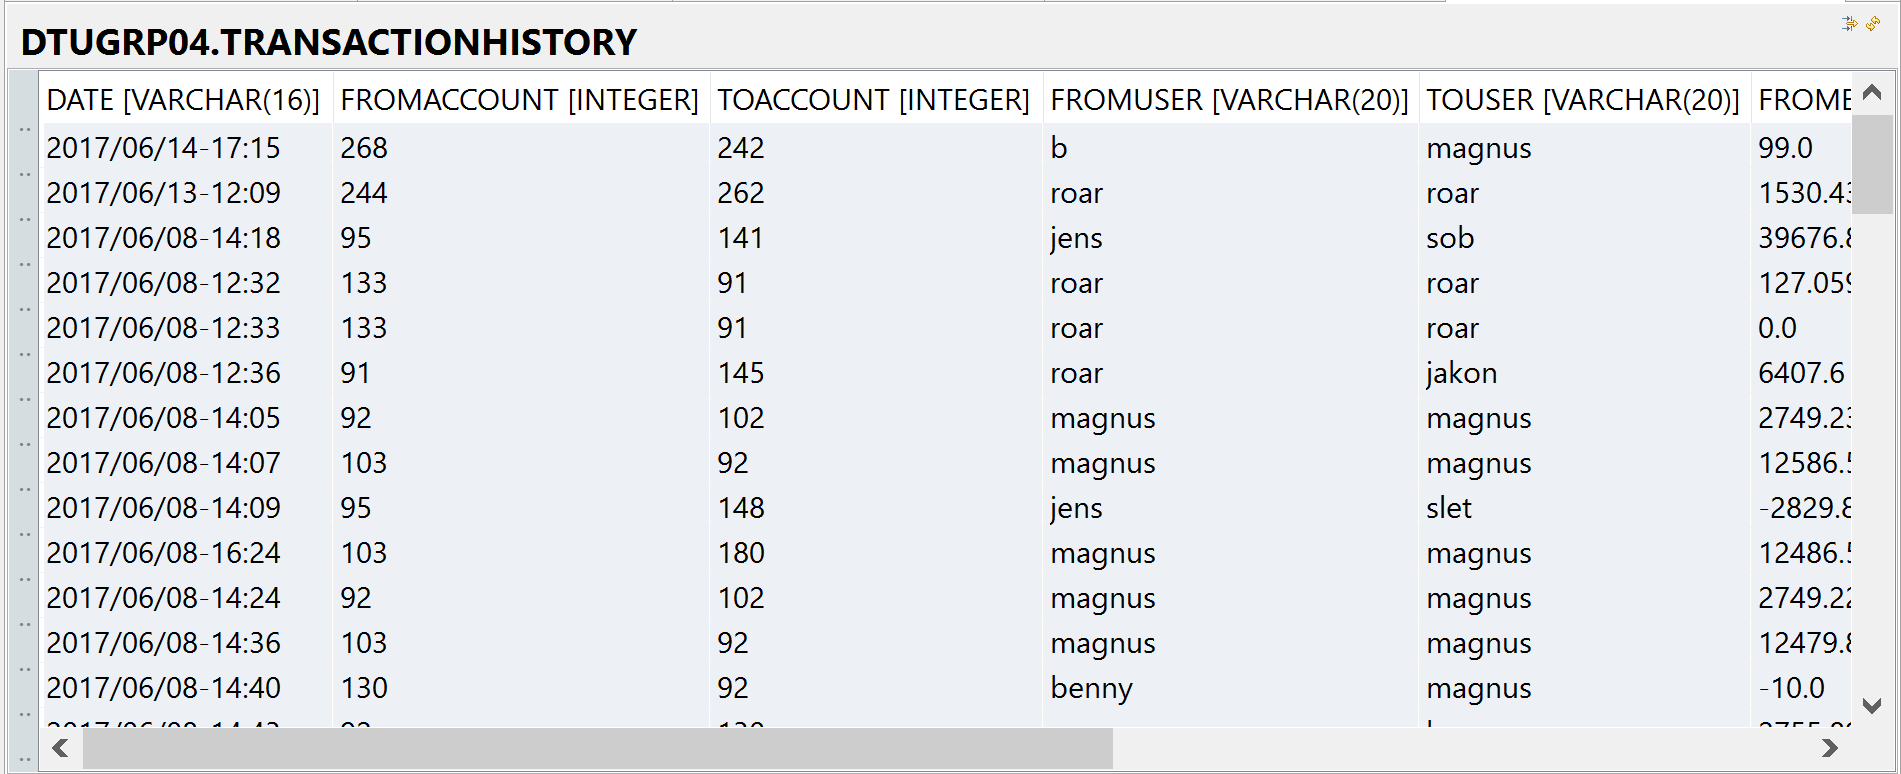
\includegraphics[width=\textwidth]{figures/transactionhistoryTable.PNG}
    \label{fig:transactionhistoryTable}
\end{figure}
\begin{figure}[H]
    \centering
    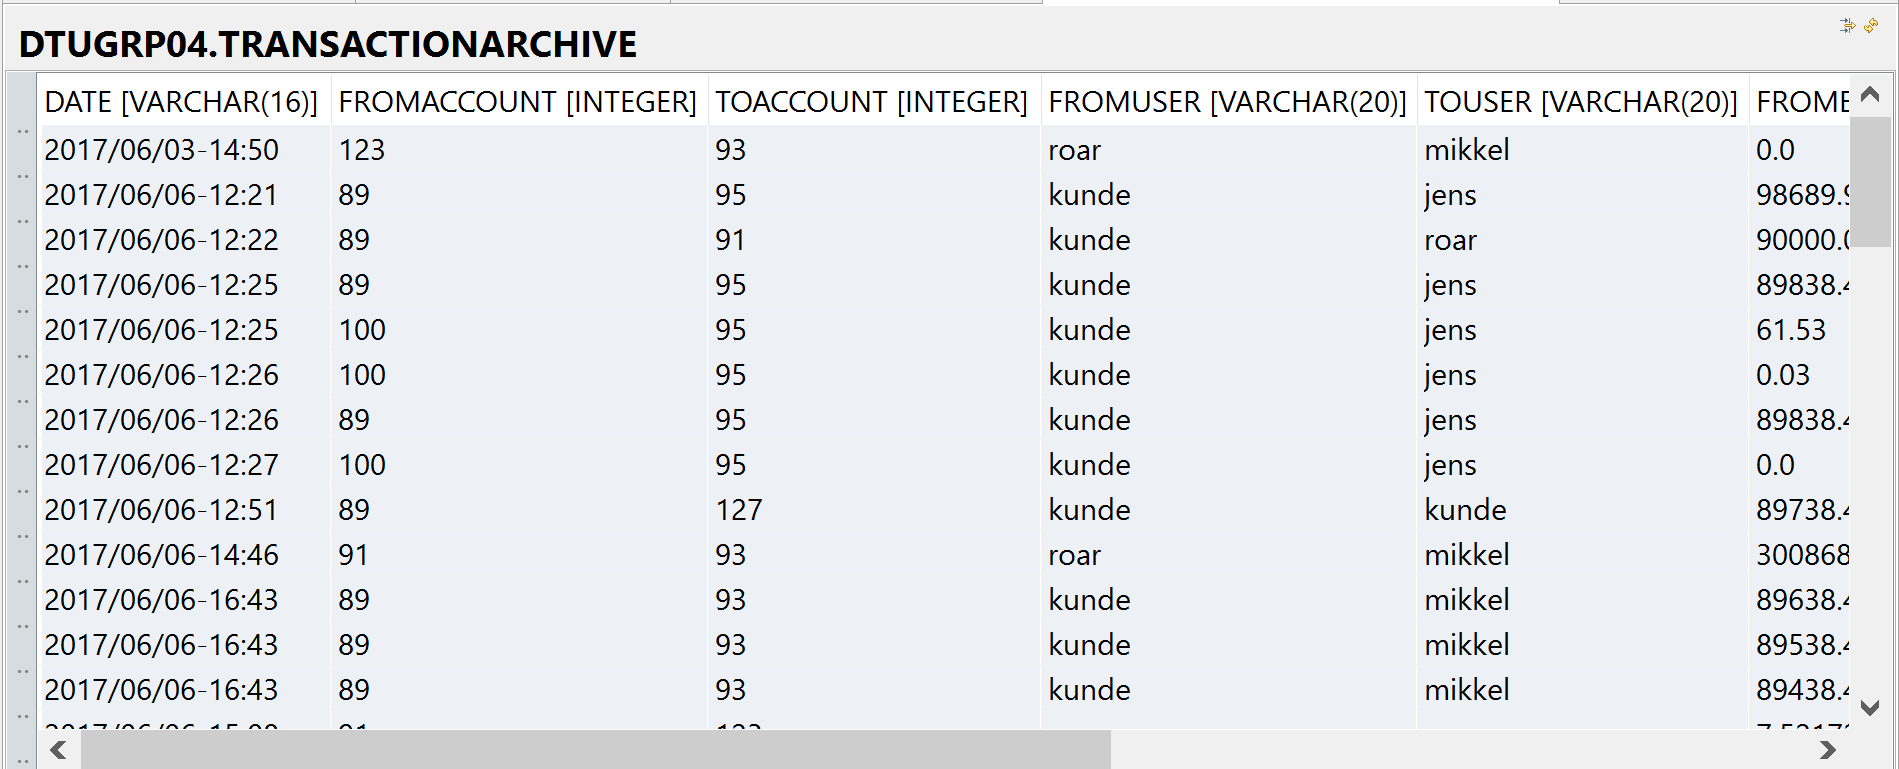
\includegraphics[width=\textwidth]{figures/transactionarchiveTable.PNG}
    \label{fig:transactionarchiveTable}
\end{figure}

%% APPENDIX END 
\end{document}
